% Created 2024-02-26 Mon 11:07
% Intended LaTeX compiler: pdflatex
\documentclass[11pt,a4paper,final]{article}
\usepackage[a4paper, total={7in, 10in}]{geometry}
\usepackage{algorithm2e}
\usepackage{booktabs}
\usepackage{subcaption}
\usepackage{graphicx}
\usepackage{tikz}
\usepackage[utf8]{inputenc}
\usepackage[T1]{fontenc}
\usepackage{graphicx}
\usepackage{longtable}
\usepackage{wrapfig}
\usepackage{rotating}
\usepackage[normalem]{ulem}
\usepackage{amsmath}
\usepackage{amssymb}
\usepackage{capt-of}
\usepackage{hyperref}
\usepackage{subfloat}                       % Subfigures
\usepackage{xcolor}                         % Color time
\usepackage{listings}                       % Code in LaTeX
\usepackage{listings-rust}                  % Code in LaTeX
\usepackage{amsfonts}                       % Cool math fonts
\usepackage{tabularx}                       % Cool tables
\usepackage{multicol}                       % Add capability to make columns
\usepackage{soul}                           % Highlight text
\usepackage{hyperref}                       % Cool clean hyperlinks
\setlength\parindent{0pt}                   % No indent for paragraphs
\lstset{language=Rust, style=boxed}
\usetikzlibrary{arrows.meta}                % Arrows for tikz
\renewcommand*{\sectionautorefname}{Section}
\renewcommand*{\subsectionautorefname}{Section}
\renewcommand*{\subsubsectionautorefname}{Section}
\renewcommand*{\paragraphautorefname}{Section}
\renewcommand*{\algorithmautorefname}{Algorithm}
\newcommand{\Or}{\textbf{ or }}
\renewcommand*{\And}{\textbf{ and }}
\newcolumntype{L}[1]{>{\hsize=#1\hsize\raggedright\arraybackslash}X}%
\newcommand{\mathcolorbox}[1]{\colorbox{yellow}{$\displaystyle #1$}}
\newcommand\mycommfont[1]{\footnotesize\ttfamily\textcolor{gray}{#1}}
\newcommand{\T}{\mathcal{T}}                % To make it clear the difference
\newcommand{\Tau}{T}                        % between Tau and T
\newcommand{\AC}{AC(u, d, v, \eta)}         % Set the parameters for AC once
\newcommand{\UC}{UC(u, d, v)}               % Set the parameters for UC once
\newcommand{\ACi}{AC(u_i, d_i, q_i, \eta_i)}% Set the parameters for AC once
\newcommand{\UCi}{UC(u_i, d_i, q_i)}        % Set the parameters for UC once
\newcommand{\Not}{\textbf{not }}            % Custom `not' operator
\newcommand{\visit}{(i, b, a, e, u, d, q, \eta, \xi)}
\newcommand{\I}{\mathbb{I}}                 % Set of visit tuples
\newcommand{\C}{\mathbb{C}}                 % Charger availability information
\newcommand{\U}{\mathcal{U}}                % Uniform distribution
\newcommand{\Sol}{\mathbb{S}}               % A shorthand for visit tuple
\newcommand{\M}{\mathbb{M}}                 % A shorthand for the metadata
\newcommand{\Hd}{\mathbb{H}}                % Set of discrete times
\newcommand{\Nu}{\mathcal{V}}               % Draw a nice Nu
\newcommand{\Iset}{I}                       % Set of visits 1-I
\newcommand{\Isetinit}{I_0}                 % Set of visits inital visits
\newcommand{\Isetfinal}{I_f}                % Set of visits final visits
\newcommand{\Bset}{B}                       % Set of visits 1-B
\newcommand{\Qset}{Q}                       % Set of visits 1-Q
\newcommand{\Jset}{J}                       % Set of visits 1-J
\newcommand{\Jsetq}{\mathbb{J}}             % Set of visits 1-J for queue active times
\newcommand{\Hset}{H}                       % Set of visits 1-H
%%-------------------------------------------------------------------------------
% Experiment parameters
\newcommand{\A}{35 }                                                            % Number of buses
\newcommand{\N}{338 }                                                           % Number of visits
\newcommand{\acharge}{0.9}                                                      % BOD charge percentage
\newcommand{\bcharge}{0.7 }                                                     % EOD charge percentage
\newcommand{\mincharge}{25\% }                                                  % Min visit charge percent
\newcommand{\minchargeD}{0.25 }                                                 % Min visit charge decimal
\newcommand{\maxcharge}{100\% }                                                 % Max visit charge percent
\newcommand{\batsize}{388 }                                                     % Battery capacity
\newcommand{\fast}{15 }                                                         % Number of fast chargers
\newcommand{\slow}{15 }                                                         % Number of slow chargers
\newcommand{\fasts}{911 }                                                       % Speed of fast charger
\newcommand{\slows}{30 }                                                        % Speed of slow charger
\newcommand{\contvars}{7,511 }
\newcommand{\intvars}{328,282 }
%%-------------------------------------------------------------------------------
%% Solve output
%% Solve output
\newcommand{\timeran}{4.2 }                                                    % Time ran for MILP [s]
\author{Alexander Brown}
\date{\today}
\title{Bus Charging Schedule Simulated Annealing with MILP Constraints}
\hypersetup{
 pdfauthor={Alexander Brown},
 pdftitle={Bus Charging Schedule Simulated Annealing with MILP Constraints},
 pdfkeywords={},
 pdfsubject={},
 pdfcreator={Emacs 29.1 (Org mode 9.6.6)}, 
 pdflang={English}}
\begin{document}

\maketitle
\tableofcontents

\parskip 3mm                                % Set the vetical space between paragraphs
\let\ref\autoref                            % Redifine `\ref` as `\autoref` because lazy
\SetCommentSty{mycommfont}                  % Set the comment color

\section{Introduction}
\label{sec:introduction}
Public transportation systems are a critical component in urban areas. An increased awareness and concern of
environmental impacts of petroleum based public transportation has driven an effort to reduce the pollutant footprint
\cite{de-2014-simul-elect,xylia-2018-role-charg,guida-2017-zeeus-repor-europ,li-2016-batter-elect}. Particularly,
the electrification of public bus transportation via battery power, i.e., battery electric buses (BEBs), has received
significant attention \cite{li-2016-batter-elect}. Although the technology provides benefits beyond reduction in
emissions, such as lower driving costs, lower maintenance costs, and reduced vehicle noise, battery powered systems
introduce new challenges such as larger upfront costs, and potentially several hours long ``refueling'' periods
\cite{xylia-2018-role-charg,li-2016-batter-elect}. Furthermore, the problem is exacerbated by the constraints of the
transit schedule to which the fleet must adhere, the limited amount of chargers available, and the adverse affects in
the health of the battery due to fast charging \cite{lutsey-2019-updat-elect}.

BEBs have been in service for many major markets, North America, Europe, and China, for more than a decade with expected
growth in the near future \cite{deng-2021-survey-elect}. The Asia Pacific market is forecasted to dominate the sales
and some major companies of the industry have also begun to enter the global market such as Volvo, BYD, and Proterra by
2025 \cite{deng-2021-survey-elect}. Much focus has been placed on the engineering of individual BEBs, such as: battery
type, brake regenerative charging, optimal battery charging, and battery degradation \cite{chen-2008-desig-grey,abdollahi-2016-optim-batter,kuhne-2010-elect,deng-2021-survey-elect}. The interest of route scheduling, charging
fleets, and optimizing the infrastructure are problems of more recent interest and are therefore timely and increasingly
relevant problems as EV/BEBs become more commonplace \cite{hoke-2014-accoun-lithium,sebastiani-2016-evaluat-elect,wei-2018-optim-spatio}.

Literature shows an interest in solving the problem of assigning BEBs to charging queues or optimizing their
infrastructure \cite{wei-2018-optim-spatio,sebastiani-2016-evaluat-elect,hoke-2014-accoun-lithium,wang-2017-elect-vehic}. Two of the main problems that have been of recent interest are
solving the problems of route scheduling and charging fleets as well as determining the infrastructure upon which they
rely. Additionally, the prospect of solving both problems simultaneously has received much attention
\cite{wei-2018-optim-spatio,sebastiani-2016-evaluat-elect,hoke-2014-accoun-lithium,wang-2017-elect-vehic}. These
problems vary by including assignment of buses to routes \cite{rinaldi-2020-mixed-fleet,zhou-2020-collab-optim,tang-2019-robus-sched,li-2014-trans-bus}, determining whether a set of existing combustion based buses should be
replaced with BEBs \cite{zhou-2020-bi-objec,duan-2021-refor-mixed,rinaldi-2020-mixed-fleet,zhou-2020-collab-optim}, and accounting for uncertainties \cite{bie-2021-optim-elect,duan-2021-refor-mixed,tang-2019-robus-sched,ursavas-2016-optim-polic}. These problems add additional complexities that warrant
simplifications due to computational complexities. One other source, as far as the reseach for this work has shown,
describes a method of producing a BEB charge schedule wih a high fidelity while accounting for multiple charger times as
well as being able to minimize over the total charger count \cite{whitaker-2023-a-network}.

Some works assume that the charge received is proportional to the time spent on the charger
\cite{liu-2020-batter-elect,yang-2018-charg-sched}. While the linear battery dynamics is a valid assumption when the
battery SOC is below 80\% \cite{liu-2020-batter-elect}, non-linear battery dynamics can be implemented to more
accurately model the charge curve. A common way to model the non-linear battery dynamics is utilizing Constant Voltage
(CV), Constant Current (CC), and Constant Current Constant Voltage (CCCV) \cite{abdollahi-2016-optim-batter,chen-2008-desig-grey}. It has also been suggested that the dynamics can be modeled as a piecewise function containing a
linear and non-linear component from which the CV and CC models construct the linear and non-linear parts, respectively
\cite{zhang-2021-optim-elect,abdollahi-2016-optim-batter}. Others have modeled the battery dynamics as a discrete
first order dynamics model \cite{whitaker-2023-a-network}. The first-order differential system, when provided a step
input, approximates the non-linear relationship between time and SOC \cite{whitaker-2023-a-network}.

Works concerning charge planning often use a version of the vehicle scheduling problem \cite{tang-2019-robus-sched,li-2014-trans-bus,he-2020-optim-charg}. Variants of this problem address infrastructure as well as determining
existing buses that should be replaced by a BEB \cite{zhou-2020-bi-objec,duan-2021-refor-mixed,rinaldi-2020-mixed-fleet,zhou-2020-collab-optim}. Other works introduce a directed graph approach to model the flow
of BEBs \cite{whitaker-2023-a-network,liu-2020-batter-elect}, where this concept was expanded to simultaneously
accounting for multiple charger types, partial charging, non-linear battery charge profiles
\cite{whitaker-2023-a-network}. The directed graph approach provides an easy method of modeling the scheduling by
discretizing the time horizon into a sequence of nodes for each charger. The nodes represent the chargers availability
and can have a maximum of one bus at a time. The buses can flow into a node to be charged and then later can exit
allowing a new bus to enter. Another method similar to the directed graph that fits the modeling of the BEB charging
scenario is the Position Allocation Problem (PAP) \cite{qarebagh-2019-optim-sched}. The PAP is derived from the Berth
Allocation Problem (BAP) which solves the problem of scheduling a set of vessels to be berthed and serviced. The model
inputs a set of vessels arrival and service times and outputs a schedule that defines the selected berth and the time
over which it is serviced. The PAP utilizes this model and redefines its inputs to EV arrival times and outputs queues
for the EVs to be charged. While the visits remain as discrete events, the time that the BEB is on the charger is
modeled as continuous, similar to \cite{frojan-2015-contin-berth,qarebagh-2019-optim-sched,zhou-2020-collab-optim}. Due to the close relationship between the BAP and PAP, BAP
literature may be used for the PAP. The literature shows methods of handling multiple quays (sets of chargers) to handle
general berthing scenarios \cite{frojan-2015-contin-berth,dai-2008-suppl-chain-analy}. Heuristic procedures for
quicker solve times have also been introduced \cite{imai-2001-dynam-berth}. Methods of defining static (full time
horizon) and dynamic (rolling-time horizon) models have been created for daily and real-time solutions, respectively,
and even fuzzy set theory has been applied to allow for more flexible schedules \cite{bello-2019-fuzzy-activ,dai-2008-suppl-chain-analy,buhrkal-2011-model-discr,frojan-2015-contin-berth}.

In what follows, the problem statement shall be provided in \ref{sec:problem-description}. \ref{sec:optimization-problem}
introduces the structure of the MILP formulation as well as a description of the parameters, decision variables,
objective function and constraints. In \ref{sec:simulated-annealing}, the concept and theory of SA is introduced. In
particular the algorithms and methods utilized for the SA implementation for this work are discussed.
\ref{sec:optimization-algorithm} outlines a generic SA algorithm, and then combines the previous sections to introduce the
particular implementation for the SA-PAP. In \ref{sec:example}, an example problem is provided to demonstrate the capability
of the work provided in this paper. The results will be presented and discussed.
\section{Problem Description}
\label{sec:problem-description}
This section introduces and defines the problem to be addressed by this work. A general description is given and
followed by a mathematical interpretation. The scope of this work will also be provided as well as a high level
introduction to the individual problems that will be addressed in order to achieve the proposed goal.

Consider a fleet of BEBs scheduled to perform a set of prescribed routes on a given day. Suppose that an individual BEB
from said fleet begins and completes an individual route at the same station from which it also receives its charge.
During each route, the BEB's State of Charge (SOC) depletes by a certain amount. The charge supplied during its visit
must be enough that it sustains the BEB's SOC at an appropriate level such that it may complete its next route. The
charge may be supplied from any single charger given a set of chargers at the station. Each time the BEB arrives at the
station, let that be denoted as an ``arrival''. Once the BEB has awaited its predetermined time (whether it has received a
charge or not), and departs from the station, let that be denoted as a ``visit''. Generalizing this to all BEBs, each BEB
will have a set of prescribed routes from which their SOC is depleted by some amount. Once their respective routes are
completed, each BEB arrives at the station to receive a charge that is sufficient to complete the next route. Each BEB
may have multiple visits to the station throughout their working day. This paper describes a method to optimize the
assignment of each visit to a charger given a schedule for a fleet of BEBs that follow the behavior described above. The
model presented in this work optimizes over power and energy consumption, as well as attempts to optimize the amount of
chargers utilized.

Consider a fleet of \(n_B\) BEBs that collectively visit a station \(n_V\) times. At said station, let there exist a pool of
\(n_Q\) charging queues from which a visiting BEB may be assigned. Let \(\mathbb{Z}\) define the set of integers. The set of arrivals
is denoted as \(\Iset = \{ 1, ... n_V \} \subset \mathbb{Z}\). Each BEB is provided an identification number \(B = \{ 1, ..., n_B \} \subset \mathbb{Z}\).
Each visit can be represented by the tuple: \(\visit\), in which the elements within the tuple denote the visit index, \(i
\in I\), BEB identification number, \(b \in B\), arrival time to the station, \(a \in \mathbb{R}\), departure time from the station, \(e \in
\mathbb{R}\), initial charge time, \(u \in \mathbb{R}\), final charge time, \(d \in \mathbb{R}\), the charger queue for the BEB to be placed into, \(q \in Q\),
the SOC upon arrival, \(\eta \in \mathbb{R}\), and the index of the next visit for the currently visiting BEB, \(\xi \in I\). Let the ordered
set of visits be denoted as \(\I\).

For each visit, a BEB must be placed in a single queue, \(q \in \Qset\). The charger \(q\) is assumed to be either a fast
charger, slow charger, or no charger at all (denoted as an idle queue). A BEB is only allowed to be assigned to one
queue per visit; however, there may be multiple BEBs charging simultaneously across different queues. The amount of time
the BEB is allowed to charge is dictated by the scheduled arrival time and required departure time, \([a_i, e_i]\).
Partial charging is allowed; however, the SOC may not exceed the BEB battery capacity and the SOC must stay above 0$\backslash$% .
The battery dynamics in this work is modeled as linear\footnote{This is most likely going to be relabeled as non-linear. Once this version of the SA is flushed out then a
section will be added to describe the non-linear battery dynamics.}, which remains accurate up to about an SOC of 80\% charge
\cite{li-2016-batter-elect}.

Each BEB arrival, except for the last arrival for each BEB, has a paired ``route'' that the BEB must perform after the
visit. This route, as one would expect, causes the BEB to discharge by some certain amount. The estimation of the SOC
lost during its route in it of itself poses a focus of research, not of which is of this work. Thus, a simplified model
of pre-calculating an average discharge is employed. The simplified model assumes a fixed discharge rate that is
multiplied by the route duration. Let the discharge of the route for visit \(i\) be denoted as \(\Delta_i \in \mathbb{R}\). The charge
supplied is encouraged to maintain the SOC of each BEB visit above a minimum battery percentage, \(\nu_b \in [0, 1]\). By this
it is meant that the SOC of a BEB is allowed to go below \(\nu_b\kappa_b\); however, if it does, the system heavily punishes the
fitness score of schedule.

The task of this paper shall be to define a method of scheduling the set of visits \(\I\) to fulfill the minimum charge
requirements over the time horizon, \(\T\), while minimizing the cost, which can be decomposed into a utility cost and an
assignment cost. The utility cost encapsulates the consumption and demand costs, and the assignment cost encapsulates
the cost of assigning a BEB to a charger and a penalty method that punishes poor BEB assignment. An objective function
is utilized to measure the relative fitness of results and constraints are employed to ensure validity of the prescribed
schedule. Both the objective function and constraints are discussed in further detail in the proceeding section.
\section{Optimization Problem}
\label{sec:optimization-problem}
This sections introduces the problem in the form of the objective function as well MILP constraints. The objective
function is required to allow relative comparisons between candidate solutions. In the context of this formulation, the
objective function is broken down into four major components: consumption cost, demand cost, assignment cost, as well as
a penalty for under-charging a bus. The constraints ensure that candidate solutions are in the feasible region. They are
composed of a set of equations defined by decision and input variables. Decision variables are those which may be
manipulated, and are chosen in an attempt to optimize the objective function. Input variables are predefined.

The input and decision variables are introduced in \ref{sec:input-variables} and \ref{sec:decision-variables}. The
objective function is introduced in \ref{sec:objective-function}. The constraints will then be introduced in
\ref{sec:constraints}.

\subsection{Variable Definitions}
\label{sec:parameter-definitions}
This section defines the input and decision variables used by the system. The input parameters are assumed to be fixed
prior to optimizing the system. The decision variables are the values that the SA algorithm has the freedom to
manipulate.

\subsubsection{Parameters}
\label{sec:input-variables}
This section introduces the parameters used in the SA algorithm. The variables to be introduced are summarized in
\ref{tab:variables}. \(\Delta_i\) is the amount energy required to complete the bus route after visit \(i\). Because there is no route
after the last visit, the power consumed after the final visit is zero. Let the set of final visits for all BEBs be
denoted as \(\Isetfinal\), the discharge for the final visit of each BEB is defined as \(\Delta_{i \in \Isetfinal} = 0\). \(\alpha_b\) is
the initial SOC percentage of bus \(b\) at the beginning of the working day. Let \(\Isetinit\) denote the set of initial
visit indices for each BEB and let \(\Xi_i \in B\) denote the identification number of the BEB for visit \(i\). The initial SOC
for bus \(\Xi_i\) can be represented as \(\eta_{i \in \Isetinit} = \alpha_{\Xi_i} \cdot \kappa_{\Xi_i}\) where \(\kappa_{\Xi_i}\) is the battery capacity for
bus \(\Xi_i\). The rest of the values for \(\eta_i : i \in I \setminus \Isetinit\) are considered decision variables and will be further
discussed in \ref{sec:decision-variables}. The notation \(t_h\) is used to denote a discrete time which is employed to
calculate the demand cost. \(dt_h\) is the discrete time slice \(dt_h = t_h - t_{h-1}\). The cost for assigning a charger to
queue \(q \in Q\) is defined by \(\epsilon_q\). \(\xi_i\) represents the next arrival index for bus \(b_i\). In other words, suppose the ID
of each BEB is recorded in order of arrival. Further suppose that recorded list is \(\xi = \{ 2,1,3,2 \}\), using a starting
index of 1, \(\xi_1 = 4\) as that is the next visit by bus 2, the same as the first visit index. The arrival and departure
times of bus visit \(i\) to the station are denoted as \(a_i\) and \(e_i\), respectively. Lastly, \(r_q\) represents the power
supplied from the charger in queue \(q \in Q\).

\begin{table}[htbp]
\caption{\label{tab:variables}Table of variables used in the paper.}
\centering
\begin{tabularx}{\textwidth}{L{0.3} L{1.2} L{0.3} L{1.2}}
\textbf{Variable} & \textbf{Description} & \textbf{Variable} & \textbf{Description}\\[0pt]
\hline
Constants &  & Constants & \\[0pt]
\(C\) & Penalty method gain factor & \(n_B\) & Number of buses in use\\[0pt]
\(n_H\) & Number of discrete steps, \(h\), in time horizon & \(n_V\) & Number of total visits\\[0pt]
\(J(u,d,v,\eta)\) & Objective function & \(n_K\) & Number of iterations in the repetition schedule\\[0pt]
\(n_M\) & Total number of steps created by initial temperature, \(\Tau_0\), and cooling schedule & \(n_Q\) & Number of chargers\\[0pt]
\(\T\) & Time horizon &  & \\[0pt]
\hline
Input variables &  & Input Variables & \\[0pt]
\(\Delta_i\) & Discharge of visit over after visit \(i\) & \(\alpha_b\) & Initial charge percentage time for bus \(b\)\\[0pt]
\(\delta_i\) & Discharge rate for vehicle \(i\) per mile & \(\nu_b\) & Minimum charge percentage allowed for each BEB \(b \in \Bset\)\\[0pt]
\(\epsilon_q\) & Cost of using charger \(q\) & \(\kappa_b\) & Battery capacity for each BEB \(b \in \Bset\)\\[0pt]
\(\rho_i\) & Route distance after visit \(i\) & \(\xi_i\) & The next index bus \(b\) will arrive\\[0pt]
\(a_i\) & Arrival time of visit \(i\) & \(\Xi_i\) & ID for bus visit \(i\)\\[0pt]
\(t_h\) & Discrete step in time horizon & \(dt_h\) & Discrete time slice in time horizon \(dt_h = t_h - t_{h-1}\)\\[0pt]
\(k\) & Local search iteration \(k\) & \(e_i\) & Time bus visit \(i\) must exit the station\\[0pt]
\(r_q\) & Charge rate of charger \(q\) &  & \\[0pt]
\hline
Direct Decision Variables &  & Direct Decision Variables & \\[0pt]
\(u_i\) & Time to start charging for visit \(i\) & \(d_i\) & Time to detach bus from charger for visit \(i\)\\[0pt]
\(q_i\) & Assigned queue for visit \(i\) &  & \\[0pt]
Indirect Decision Variables &  & Indirect Decision Variables & \\[0pt]
\(\eta_i\) & Charge for the bus at the beginning of visit \(i\) & \(\psi_{ij}\) & Tracks spatial overlap for visit pair \((i,j)\)\\[0pt]
\(\sigma_{ij}\) & Tracks temporal overlap for visit pair \((i,j)\) & \(d_i\) & Detach time from charger for visit \(i\)\\[0pt]
\(p_{dem}(t)\) & Demand cost & \(s_i\) & Amount of time spent on charger for visit \(i\) (service time)\\[0pt]
\hline
\end{tabularx}
\end{table}

\subsubsection{Decision Variables}
\label{sec:decision-variables}
Decision variables are those chosen by the optimizer. The variables will be broken into two sections: direct and
indirect decision variables. Direct decision variables are those that the system manipulates directly, and indirect
variables are those that are influenced by the direct.

\paragraph{Direct Decision Variables}
\label{sec:direct-decision-variables}
The first two variables are \(u_i\) and \(d_i \; \forall i \in \Iset\). They represent the initial and final charging times. These
values must remain within range of the arrival and departure times, \([a_i, e_i]\), for visit \(i\). The last direct
decision variable is the queue that bus visit \(i\) can be placed in to charge, \(q_i \in \Qset\).

\paragraph{Indirect Decision Variables}
\label{sec:indirect-decision-variables}
Let the initial SOC for a visit be written as \(\eta_i\), where \(i \in \Iset \setminus \Iset_0\). The initial charge for visit \(i\) forms
the foundation from which the SOC of the next visit, \(\xi_i\), is calculated. This propagation of the SOC is evaluated as
shown in \ref{eq:bat-chain}. The equation states that the charge for bus \(i\)'s next visit is equal to the initial charge for
visit \(i\) plus the charge added to it by charger \(q_i\) over duration \(s_i = d_i - u_i\) minus the discharge accumulated
over route \(i\).

\begin{equation}
\label{eq:bat-chain}
  \eta_{\xi_i} = \eta_i + r_{q_i}s_i - \Delta_i
\end{equation}

A penalty method is to be implemented in the objective function that is enabled when the \(\eta_i\) falls below a defined
threshold. Let the piecewise function that enables/disables the penalty method be of the form \ref{eq:penalty}.

\begin{equation}
\label{eq:penalty}
  \phi(x) =
  \begin{cases}
    0   & x \ge 0 \\
    x^2 & x < 0\\
  \end{cases}
\end{equation}

If \(x = \eta_i - \nu_{\Xi_i} \kappa_{\Xi_i}\), where \(\nu_{\Xi_i} \kappa_{\Xi_i}\) is the minimum charge threshold, then \ref{eq:penalty} defines the
penalty method that encourages schedules to maintain the SOC for each visit above \(\nu_{\Xi_i} \kappa_{\Xi_i}\). If the SOC is falls
below the specified threshold, a penalty proportional to the difference of the SOC and the threshold squared is applied.

The variables \(\sigma_{ij}\) and \(\psi_{ij}\) are used to indicate whether a visit pair \((i, j)\) overlap the same space as show in
\ref{fig:spacial-and-temporal-constr}. Formally, \ref{eq:bus-spat-temp} describes the relationship that \(\sigma_{ij}\) and \(\psi_{ij}\)
uphold. That is, for every visit, if the start charge time of visit \(j\) is greater than the end charge time of visit
\(i\), then \(\sigma_{ij}\) is active (\(\sigma_{ij} = 1\)). Similarly, if the queue for visit \(j\) is in a queue that is in a queue of a
greater index than visit \(i\), then \(\psi_{ij}\) is active (\(\psi_{ij} = 1\)). These variables will be further elaborated on in
\ref{sec:constraints}.

\begin{subequations}
\label{eq:bus-spat-temp}
\begin{equation}
  \sigma_{ij} =
  \begin{cases}
    1 & \text{if } u_i \ge d_j, \; i \ne j\\
    0 & \text{otherwise}
  \end{cases}
\end{equation}

\begin{equation}
  \psi_{ij} =
  \begin{cases}
    1 & \text{if } q_i \ge q_j,\; i \ne j\\
    0 & \text{otherwise}
  \end{cases}
\end{equation}
\end{subequations}

The demand cost, \(p_d\), of the charging schedule. It is calculated after all the decision variables have been assigned.

\subsection{Objective Function}
\label{sec:objective-function}
The objective function is used to compare the relative fitness of different candidate solutions against one another.
This objective function takes in input and decision variables to calculate some value of measure. The calculated
objective function value can either be maximized or minimized; the desired option is dependent on the problem to be
solved as well as the formulation of said objective function. Let \(J\) represent the objective function. The objective
function for this problem has four main considerations: charger assignment, consumption cost, demand cost, and penalty
on insufficient charge. These considerations are divided into two components: The assignment cost and the utility cost.

Suppose the objective function is of the form \(\text{min } J = \AC + \UC\). \(\AC\) is the assignment cost, and \(\UC\) is
the utility cost. The assignment cost represents the costs of assigning a bus to a particular queue as well as the
chosen charging period, \([u_i, d_i]\). The assignment cost increases is cost as the selected index increases and the cost
of the chosen charge times is implemented by utilizing a penalty method. The penalty method assigns a high cost to the
system if it falls below a specified SOC threshold. The assignment cost is defined as

\begin{equation}
\label{eq:ac}
\AC = \sum_{i=1}^{n_V} \Big(\epsilon_{q_i}r_{q_i} + C \phi_i(\eta_i - \nu_{\Xi_i} \kappa_{\Xi_i}) \Big)\text{.}
\end{equation}

The first term in the summation represents the calculation of the cost for assigning a bus to queue \(q \in Q\). Let \(\epsilon\) be
a vector of the form \(\epsilon = [100, 200, ..., 100n_Q]\). When written in this way, \(\epsilon\) encourages the objective function to
minimize the total amount of chargers. Iterating on this concept, let the first \(n_B\) indices to be idle queues (i.e.
queues in which no charge is supplied), the next \(n_{Q_s}\) indices to be slow chargers, and the next \(n_{Q_f}\) indices
to be fast chargers, where \(n_B, n_{Q_s}, n_{Q_f} \in \mathcal{Z}\) and \(n_B + n_{Q_s} + n_{Q_f} = n_Q\). The \(\epsilon\) vector thus be
concatenated as follows: \(\epsilon = [[\mathbf{0}; n_B], [100, 200, ..., 100n_Q]]\), where \(\mathbf{0}_{n_B}\) indicates a zero
vector of length \(n_B\). That is, \(\epsilon_{q_i}\) has no cost if \(q_i \le n_B\) or is incrementally penalized as the selected
queue index increases if \(n_B < q_i \le n_B + n_{Q_s} + n_{Q_f}\). In words, this form accrues no cost when assigning a BEB
to an idle queue while still minimizing charger count and encouraging the use of slow chargers over fast. While the \(\epsilon\)
vector can be constructed in many other ways, the form shown above is the method applied to this work.

The second term is the penalty function that is either enabled or disabled by \(\phi_i\)
\cite{luenberger-2008-penal-barrier-method}. The penalty function is enabled, \(\phi_i = (\eta_i - \nu_{\Xi_i} \kappa_{\Xi_i})^2\), if the
SOC falls below a specified threshold, \(\eta_i \le \nu_{\Xi_i} \kappa_{\Xi_i}\), and is disabled, \(\phi_i = 0\), otherwise. This term is
considered an assignment cost because the penalty method is enabled due to poor allocations of BEBs. That is, the cost
is not impacted by how much the system consumes energy, but by how the BEBs have been assigned. \(C\) is a large constant
value used to scale the penalty function.

The utility cost is composed of the consumption cost and the demand cost. The consumption cost is merely the summation
of all the energy being used over all the active periods for each charger in the time horizon, \(\sum_{i=1}^{n_V}
r_{q_i}s_i\). That is, the charge rate, \(r_{q_i}\), for the active charger, \(q_i\), is multiplied by the time that the
charger will be utilized, \(s_i\).

The demand cost quantifies the amount of power being used over a given period of time and increases the cost if too much
power is utilized within said period. A typical period in which to calculate the demand cost is over 15 minute
increments (900 seconds). Let the average power used over an arbitrary 15-minute interval be represented by \ref{eq:p15}.

\begin{equation}
\label{eq:p15}
p_{15}(t) = 900 \int_{t-900}^{t} p(\tau) d\tau
\end{equation}

Worst case must be assumed to ensure enough power is available during peak hours; therefore, the maximum value found is
retained.

\begin{equation}
\label{eq:pmax}
p_{max}(t) = \max\limits_{\tau \in [0,t]}p_{15}(\tau)
\end{equation}

\ref{eq:pmax} is thus a function that describes the largest demand cost found up to time \(t\). A fixed minimum average power is
introduced that is intended to act as a base threshold before the cost begins to increase. Let this fixed threshold be
defined as \(p_{fix}\). Furthermore, let \(z\) define the demand rate which has the units of \(\frac{\$}{kW}\).

\begin{equation}
\label{eq:pdem}
p_d(t) = \max(p_{fix},p_{max}(t))z
\end{equation}

Hence, \ref{eq:pdem} begins with a value of \(p_{fix}\) from which it may only increase if \(p_{15}(t) > p_{fix}\). Let \(h \in \{ 1,
2, ..., n_H \} \subset \mathcal{Z}\) and \(n_H = \frac{T}{900}\). Furthermore, let \(p\) define the vector of discrete power consumption and
let \(p_h \in p\) be the discrete power demand at time step \(h\). For conciseness of notation we will abuse \(t_h\) to denote
the time in discrete form (as opposed to \(t\) being continuous), let \(dt_h = t_h - t_{h-1}\), and \(\Hset = \{ 1, 2, ...,
n_H \}\). Knowing the charger speed, \(r_{q_i}\), and the initial and final charge times, \(u_i\) and \(d_i\), respectively.
The corresponding discrete indices of \(h \in \Hset\) for the range \([u_i, d_i]\) can be determined by first calculating the
total number of steps in the range \(n_h = \frac{d_i - u_i}{dt}\). Once the number of steps are know, the consumed power,
\(r_{vi}\) can be added to the correct indices in \(p\). This procedure is outlined in \ref{alg:calc-p}.

\begin{algorithm}[H]
\caption{Calculate $p$} \label{alg:calc-p}
\LinesNumbered
\TitleOfAlgo{Calculate $p$}
\KwIn{$(\I, r)$}
\KwOut{$p$}

\Begin
{
  $dt \leftarrow 900$\tcc*{Creat time step of 15 minutes}
  $p \leftarrow [0.0; n_H]$\tcc*{Allocate an $n_H \times 1$ vector filled with zeros}

  \tcc{For each visit}
  \ForEach {$\I_i \in \I$}
  {
    $n_h \leftarrow \frac{\I_{i.d} - \I_{i.u}}{dt}$\tcc*{Calculate the total number of steps in the time slice}

    \tcc{For each index in the time slice $[u_i, d_i]$}
    \ForEach {$h \in \{\frac{u_i}{dt}, \frac{u_i + dt}{dt}, ..., \frac{u_i + n_h dt}{dt}\}$}
    {
      $p[h] \leftarrow p[h] + r_{\I_{i.q}}$\tcc*{Add the consumed power during discrete step}
    }
  }
  \Return{$p$}
}
\end{algorithm}

With the consumed power calculated for each time step, the peak 15 for each interval in the time horizon can be written
as follows.

\begin{equation}
p_{15}[h] = \sum_{h-\frac{900}{dt}+1}^h p_h,
\end{equation}

where \(15 \le h \le n_H\). Similarly to before, the maximum \(p_{15}[h]\) value is to be retained via \(p_{max} = \max\limits_{h
\in H}p_{15}[h]\). Thus, the discrete demand cost is expressed as shown in \ref{eq:pd-dis}.

\begin{equation}
\label{eq:pd-dis}
  p_d = \max(p_{fix}, p_{max})z
\end{equation}

To write the utility cost the consumption and \ref{eq:pd-dis} are added together to create \ref{eq:pc}.

\begin{equation}
\label{eq:pc}
\UC = p_d + \sum_{i=1}^I \Big( r_{q_i}s_i \Big)
\end{equation}

\subsection{Constraints}
\label{sec:constraints}
Now that a method of calculating the fitness of a schedule has been established, a method for determining the
feasibility of a schedule must be defined. The feasible space for schedules defines the space in which the input and
decision variables describe a schedule that would keep the BEBs adequately charged throughout the working day while
maintaining their route schedules. To ensure the selected decision variables fall within the feasible space, a set of
constraints are applied to a given candidate solution. The constraints must ensure no overlap temporally or spatially,
the BEB must receive enough charge to complete its next route, the BEB cannot be over-charged, and the BEB must depart
on time. The aforementioned constraints are shown in \ref{eq:constraints}.

\begin{multicols}{2}
\begin{subequations}
\label{eq:constraints}

  \begin{equation}
      \label{seq:c0}
      u_j - d_i - (\sigma_{ij} - 1)T \ge 0
  \end{equation}
  \begin{equation}
      \label{seq:c1}
      q_j - q_i - 1 - (\psi_{ij} - 1)Q \ge 0
  \end{equation}
  \begin{equation}
      \label{seq:c2}
      \sigma_{ij} + \sigma_{ji} \le 1
  \end{equation}
  \begin{equation}
     \label{seq:c3}
      \psi_{ij} + \psi_{ji} \le 1
  \end{equation}
  \begin{equation}
      \label{seq:c4}
      \sigma_{ij} + \sigma_{ji} + \psi_{ij} + \psi_{ji} \ge 1
  \end{equation}
  \begin{equation}
      \label{seq:c5}
      s_i = d_i - u_i
  \end{equation}
  \begin{equation}
      \label{seq:c6}
       \eta_{\xi_i} = \eta_{i} + r_{q_i}s_i - \Delta_i
  \end{equation}
  \begin{equation}
      \label{seq:c7}
      \kappa_{\Xi_i} \geq \eta_{i} + r_{q_i}s_i
  \end{equation}
  \begin{equation}
      \label{seq:c8}
      a_i \leq u_i \leq d_i \le e_i \le \T
  \end{equation}
\end{subequations}
\end{multicols}

Constraints \ref{seq:c0}-\ref{seq:c4} are the ``queuing constraints''. They are preventing overlap both spatially and
temporally as shown in \ref{fig:spacial-and-temporal-constr}. The y-axis represents the possible queues for a bus visit to be
placed into, and the x-axis represents the time that can be reserved for each visit. The shaded rectangles represent
time that has been scheduled in the horizontal direction, and the queue allocated for each bus visit in the vertical
direction. In other words, the set of constraints \ref{seq:c0} - \ref{seq:c4} aim to ensure that these shaded rectangles
never overlap.

\begin{figure}[ht!]
  \centering
  \scalebox{0.5}{
  \centerline{
    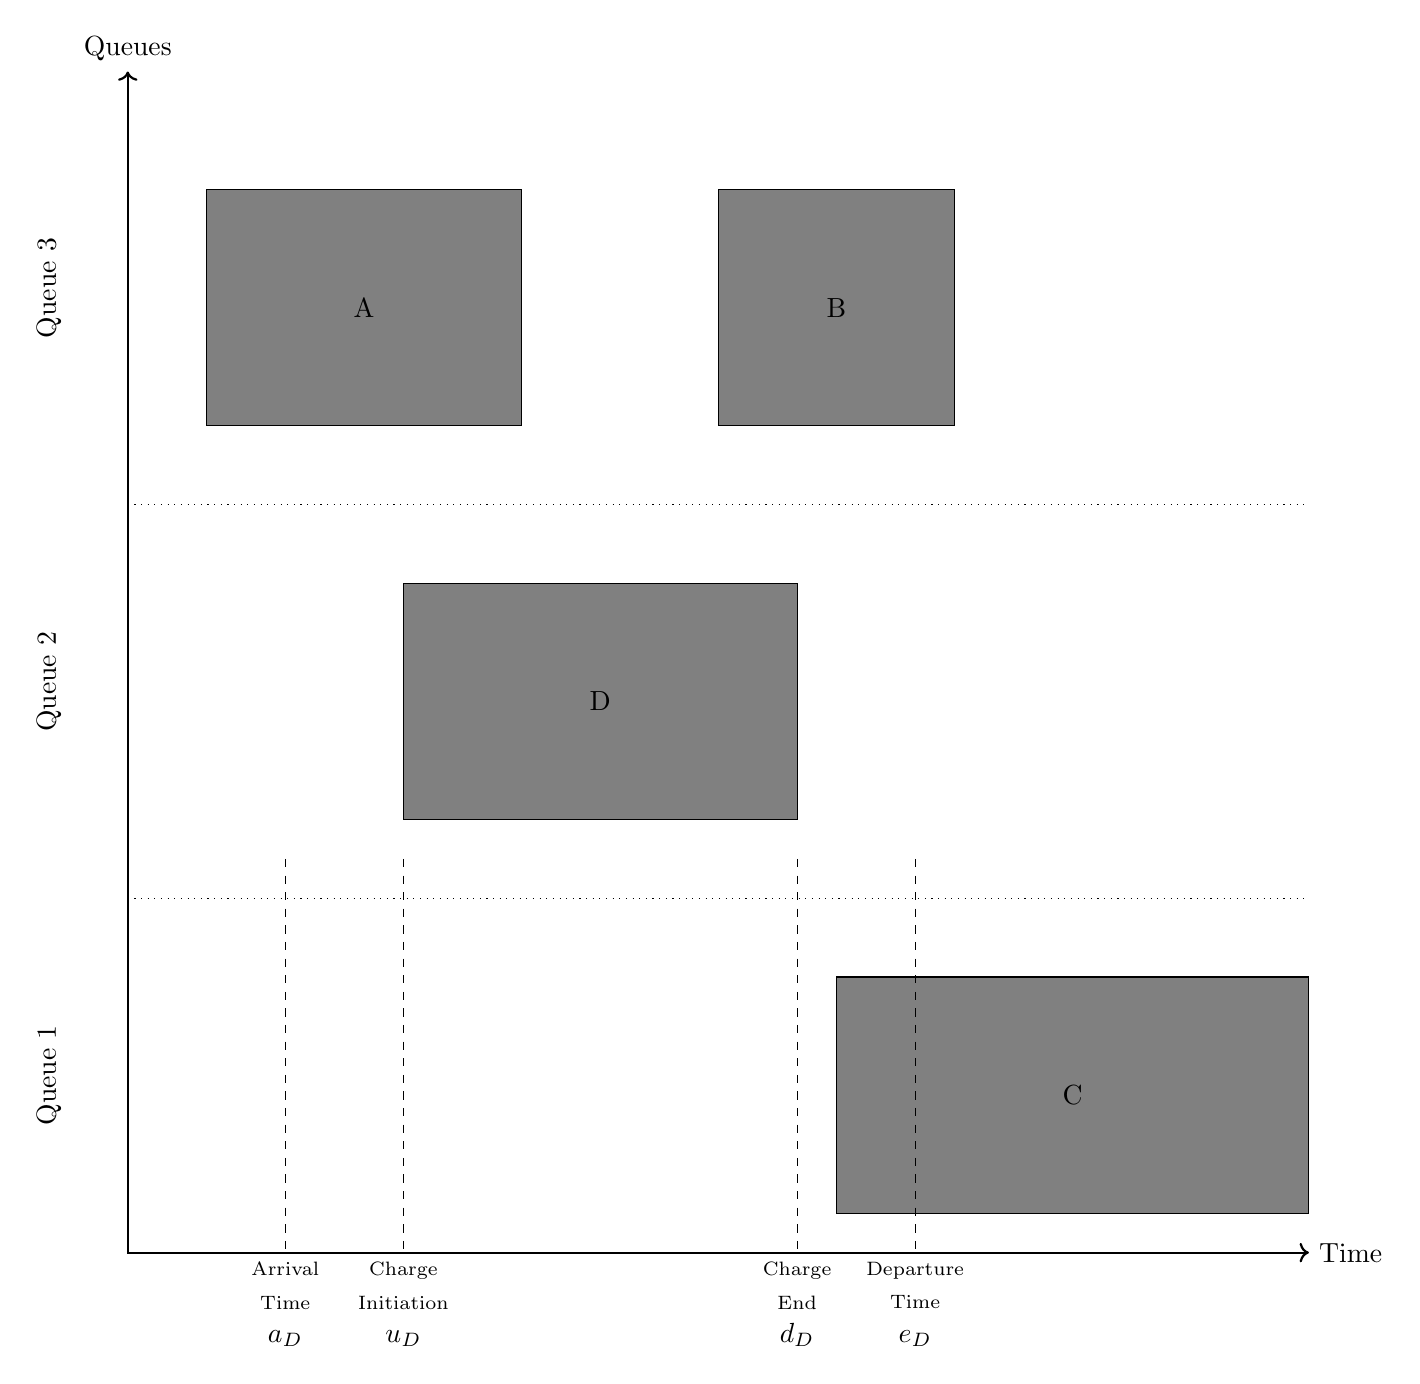
\begin{tikzpicture}
      % Variables
      \def \arrx   {2.0}
      \def \initx  {3.5}
      \def \endx   {8.5}
      \def \depx   {10.0}
      \def \yshift {5}

      % Axis
      \draw [thick,<->] (0,15) node[above]{Queues} -- (0,0) -- (15,0) node[right]{Time};

      % Rectangles
      \node[rectangle, draw, fill=gray, minimum width=4cm, minimum height = 3cm] at (3,12) {A};
      \node[rectangle, draw, fill=gray, minimum width=3cm, minimum height = 3cm] at (9,12) {B};
      \node[rectangle, draw, fill=gray, minimum width=5cm, minimum height = 3cm] at (6,7) {D};
      \node[rectangle, draw, fill=gray, minimum width=6cm, minimum height = 3cm] at (12,2) {C};

      % X-axis labels
      \node [below,align=center] at (\arrx,0) {\scriptsize Arrival     \\ \scriptsize Time \\ $a_D$};
      \node [below, align=center] at (\initx,0) {\scriptsize Charge    \\ \scriptsize Initiation  \\ $u_D$};
      \node [below, align=center] at (\endx,0) {\scriptsize Charge     \\ \scriptsize End \\ $d_D$};
      \node [below, align=center] at (\depx,0) {\scriptsize Departure  \\ \scriptsize Time \\ $e_D$};

      % Y-axis labels
      \node[rotate=90] at (-1, 2.25) {Queue 1};
      \node[rotate=90] at (-1, 7.25) {Queue 2};
      \node[rotate=90] at (-1, 12.25) {Queue 3};

      % Vertical lines
      \draw[dashed] (\arrx,\yshift)--(\arrx,0);
      \draw[dashed] (\initx,\yshift)--(\initx,0);
      \draw[dashed] (\endx,\yshift)--(\endx,0);
      \draw[dashed] (\depx,\yshift)--(\depx,0);

      % Horizontal lines
      \draw[dotted] (0, 4.5) -- (15, 4.5);
      \draw[dotted] (0, 9.5) -- (15, 9.5);

    \end{tikzpicture}
  }}
  \caption{The representation of the queue-time space. The x and y-axis represent time and space, respectively. Along the y-axis, the dashed lines represent discrete queuing locations. The shaded rectangles represent schedules BEBs to be charged. The height of each shaded rectangle represents the space taken on the queue and the width being the time to service said BEB. The vertical dashed lines are associated with vessel D and represent the arrival time, initial charge time, charge completion time, and departure time. Note that the arrival time may be before the initial charge time and the completion time may before the departure time.}
  \label{fig:spacial-and-temporal-constr}
\end{figure}

Constraint \ref{seq:c4} states that the starting service time for BEB \(i\), \(u_j\), must begin after the previous BEB
departs, \(d_i\). The last term utilizes big-M notation to activate or deactivate the constraint. A value of \(\sigma_{ij} = 1\)
will activate the constraint to ensure that bus \(i\) is complete before bus \(j\) is allowed to begin being serviced. If
\(\sigma_{ij} = 0\), then the constraint is of the form \(T + d_j > u_i\) rendering the constraint ``inactive'' because \(u_i\)
cannot be larger than \(d_i\). This effectively allows the charging windows of the vehicle to overlap. This is important when the BEBs are not in the same queue.

Similarly, \(\psi_{ij}\) determines whether the vehicles are charging in the same queue. If \(\psi_{ij} = 1\) then \eqref{seq:c1}
is active; thus, vehicle \(i\) is in a queue index that is less than BEB \(j\). If \(\psi_{ij} = 0\) then the constraint is
deactivated and BEB \(i\) is in a queue index greater than that of BEB \(j\).

 \ref{seq:c5} describes the service time of the bus. \ref{seq:c6} calculates the initial charge for the next visit for
bus \(b_i\). \ref{seq:c7} ensures that the bus is not being over-charged. \ref{seq:c8} ensures the continuity of the times
(i.e. the arrival time is less than the initial charge which is less than the detach time which is less than the time
the bus exits the station and all must be less than the time horizon).
\section{Simulated Annealing}
\label{sec:simulated-annealing}
SA is a well-studied local search metaheuristic used to solve discrete and (to a lesser degree) continuous problem
\cite{gendreau-2018-handb-metah}. A metaheuristic is a high-level problem-independent algorithm framework that provides
a set of guidelines or strategies to develop heuristic optimization algorithms \cite{radosavljevic-2018-metah-optim}.
Metaheuristic problems primarily fit in two categories: population-based and single-solution-based. Population based
algorithms emphasize exploration of the solution space as apposed to single-solutions-based algorithms being more
exploitation oriented \cite{radosavljevic-2018-metah-optim}. Generally, metaheuristic algorithms share the basic
advantage of speed in finding a satisfactory solution for large-scale practical optimization problems
\cite{radosavljevic-2018-metah-optim}. SA, however, is sometimes criticized for the speed at which it converges to the
global optimum \cite{gendreau-2018-handb-metah,henderson-1989-theor-pract}.

SA is an exploitation oriented, single-solution based metaheuristic. In addition to the advantages of simplicity, both
theoretically and implementation, the algorithm has an inherent ability to overcome non-linearities
\cite{gendreau-2018-handb-metah,radosavljevic-2018-metah-optim}. This model is named after its analogized process
where a crystalline solid is heated then allowed to cool at a slow rate until it achieves its most regular possible
crystal lattice configuration \cite{henderson-1989-theor-pract}. SA establishes a connection between this thermodynamic
process and the search for global optima in optimization problems.

There are five key components to SA: initial temperature, cooling schedule (temperature function), generation
mechanisms, acceptance criteria, and a local search iteration count (temperature change counter)
\cite{keller-2019-multi-objec}. The temperature function describes the speed at which the system is ``cooled'' over each
iteration. The generation mechanisms provide a means of modifying the system by some singular discrete change that is
within the neighborhood of the previous solution \cite{gendreau-2018-handb-metah}. The acceptance criteria is a
function of the system temperature that makes the decision whether the system will accept an inferior solution in favor
of exploring the solution space. Finally, the local search iteration count is the number of steps taken to try to
exploit a solution at a constant temperature. Each of these mechanisms are elaborated in the subsequent sections.

\subsection{Cooling Equation}
\label{cooling-equation-experimental}
The temperature function models a ``rate of cooling'' for the SA process. Initially, when the temperature is high, SA
encourages exploration. As the process begins to ``cools down'' (in accordance to the cooling schedule), it begins to
encourage local exploitation of the solution (rather than exploration)
\cite{rutenbar-1989-simul-anneal-algor,henderson-1989-theor-pract}. There are three common basic types of cooling
equations: linear, geometric, and exponential. Each schedule is depicted in \ref{fig:cool} \cite{keller-2019-multi-objec}.
Every plot begin with an initial temperature of \(T_0 = 500^\circ\; C\) and a final temperature of \(T_f = 1^\circ\; C\). The
different cooling schedules dictate the rate at which the algorithm progressively disallows exploration. Let the vector
of temperatures described by a cooling schedule be defined as \(t\). Furthermore, let an element of the vector be denoted
as \(t_m \in t\), where \(m \in [0,...,M]\) and \(M = \lvert t \rvert\). A linear cooling schedule is defined by \ref{eq:cool0}.

\begin{equation}
\label{eq:cool0}
t_m = t_{m-1} - \delta_0
\end{equation}

with \(t_0 = \Tau_0\) and \(\delta_0 = 1/2\; C^\circ\) in \ref{fig:cool}. The value of \(\delta_0\) may vary anywhere in the range \(\delta_0 \in \mathbb{R}^+\). A
geometric cooling schedules is as defined in \ref{eq:cool1}. This schedule type is most widely used in practice
\cite{keller-2019-multi-objec}. As such, it will also be employed by the work in this paper.

\begin{equation}
\label{eq:cool1}
t_m = \delta t_{m-1}
\end{equation}

where \(\delta = 0.995\) in \ref{fig:cool}. The gain variable, \(\delta\), may vary anywhere between the range \([0,1)\). An exponential
cooling schedule is defined by the difference equation as shown in \ref{eq:cool2}.

\begin{equation}
\label{eq:cool2}
t_m = e^{-\delta}t_{m-1}
\end{equation}

where \(\delta = 0.01\) in \ref{fig:cool}. A typical range for \(\delta\) is \(0.8 \le \delta \le 0.99\) \cite{delahaye-2019-simul}.

\begin{figure}[htbp]
\centering
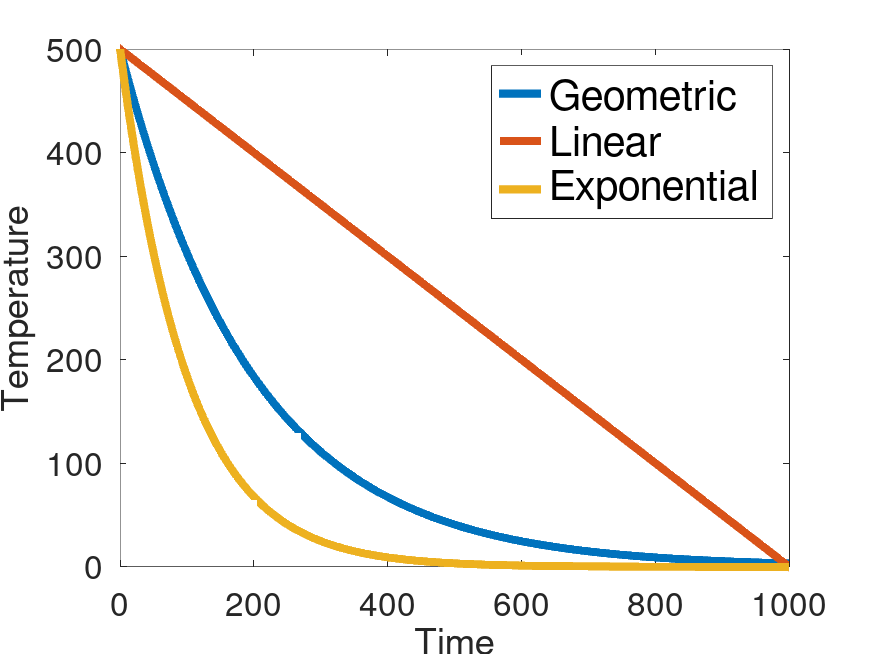
\includegraphics[width=0.5\textwidth]{sections/img/cool_func.png}
\caption{\label{fig:cool}Cooling equations}
\end{figure}

\subsection{Acceptance Criteria}
\label{sec:acceptance}
In SA, the algorithm stores a candidate solution that is continuously compared to newly generated solutions. Let the
stored solution be referred to as the ``active solution''. During each iteration, a new candidate solution is generated
and compared to the active solution to determine if the new solution should replace the active solution. In order to
determine if the active solution is to be replaced, an acceptance criteria is defined. A new candidate solution that is
more fit than active solution (fitness being dictated by the objective function) is always accepted as the new active
solution. In an effort to encourage exploration, inferior candidate solutions have a probability of being accepted as
the active solution. The probability of accepting an inferior candidate solution is described by the function
\(\exp(-\frac{J(x) - J(\bar{x})}{t_m})\) where \(J(\cdot)\) is the objective functions described in \ref{sec:objective-function},
\(t_m\) is current temperature, \(x\) is the current solution, and \(\bar{x}\) is the new candidate solution. The probability
of acceptance is a function of the current temperature and the difference of the active solution and a new candidate
solution. Formally, let \(\Delta E \equiv J(x) - J(\bar{x})\) and let \(f(\cdot)\) be the function that describes the probability of
accepting a candidate solution \(\bar{x}\). The acceptance of a candidate solution is thus of the form shown in
\ref{eq:candaccept} \cite{keller-2019-multi-objec}.

\begin{equation}
\label{eq:candaccept}
f(x,\bar{x},t_m) =
\begin{cases}
  1                   & \Delta E > 0 \\
  e^{- \frac{\Delta E}{t_m}} & \text{otherwise}
\end{cases}
\end{equation}

\subsection{Generation Mechanisms}
\label{sec:generation-mechanisms}
Generation mechanisms are used to create a neighboring candidate solution \cite{gendreau-2018-handb-metah}. That is,
the generating function creates a solution that can be reached in a single iteration from the active solution. In the
case of the problem statement made in \ref{sec:problem-description}, six primitive generation mechanism shall be used: new
visit, slide visit, new charger, new window, wait, and purge. The purpose of each of these generators is to assign new
visits to a charger, adjust a bus visits initial and final charge time within the same time frame/queue, move a BEB from
one charger to another with the same charge schedule, move a bus to its idle queue, and remove a charger from the set
of charger availability's. Each generator will be discussed in more detail in \ref{sec:generators}.

These generation mechanisms will in turn be utilized by two wrapper functions. The schedule generation is to used create
an initial candidate solutions for SA to compare with other solutions, and the perturb schedule generator is used to
take a candidate solution and alter it slightly in an attempt to step toward a global or local minimum. The wrapper
functions will be discussed in \ref{sec:generator-wrappers}. However, prior to discussing the primitives and wrapper
generating functions, their respective inputs and outputs must be defined.

\subsubsection{Generator Input/Output}
\label{sec:generator-input-output}
This section discusses in detail the expected inputs and outputs of each generator. It is important to discuss these
parameters to have an understanding of the generator algorithms to be derived. The input consists of the bus visit index
of interest, information about the current state of visits, \(\I\), and the current state of the charger availability,
\(\C\). The availability of each charger, \(\C\), is iteratively constructed throughout the SA process. The output of each
generator affects the tuple (or a subset of the tuple) of decision variables \((q_i, u_i, d_i)\) and charger availability
\(\C\).

In the development of the algorithms, dot notation is to be introduced to extract variables from tuples. For example,
suppose the arrival time is desired to be extracted from visit \(i\). Given \(\Sol\), the notation that describes extracting
the initial visit \(u_i\) is written as \(u_i \equiv \I_{i.u}\).

\paragraph{Generator Input}
\label{sec:org5d953fb}
Each generator accepts an input of the tuple of the form \(\Sol \equiv (i, \I, \C)\) where \(i\) is the visit index being
manipulated, \(\I\) is the tuple that describes the set of visits, and \(\C\) is the set that describes the availability for
all chargers \(q \in \Qset\). In other words, \(\C\) defines the set of times when the chargers are not being utilized or are
``inactive''.

To derive \(\C\), consider its complement, \(\C'\), which is the set of ``active'' time periods for each charger. Let \(\C_q' \subset
\C'\) describes the active times for charger \(q\). Focusing on an individual charger, consider \(\C_q'\) before a schedule
has been imposed upon it, \(\C_q' = \{ \varnothing \}\). In other words, no buses have been assigned to be charged over
some time period \([u_i, d_i]\). After the scheduling process is complete, \(\C_q'\) will have a set of active periods of
the form \(\C_q' = \{[u_i, d_i]: i \in I\}\). With a fully defined set \(\C_q'\), its compliment can be found, \(\C_q\).

Let \(i^{\text{th}}\) inactive period be denoted as \(\C_{i.q}\). To determine the inverse of \(\C_q'\), begin by noting that
\(\C_q'\) is said to be disjoint, \(\C_q' \bigcap \{[u_j, d_j] : j \in \Jsetq\} = \varnothing\) (i.e. the sets share no common
elements) \cite{halmos-1974-naive-set-theor}. The inverse of a disjoint set can be found by the De Morgan Law: \((A \cap
B)' = A' \cup B'\). Using De Morgan's Law, the set of inactive periods can be written as \(\C_q \equiv \bigcup \{[u_j, d_j]': j \in
\Jsetq\}\).

\paragraph{Generator Output}
\label{sec:orge3f1d05}
The output of the generating functions is the same as the input, \(\Sol\), but with changes applied to it by a generator.
Let a modified variable be denoted with a bar, \(\bar{\cdot}\). Thus, the modified input tuple is written as \(\bar{\Sol}\).
Although not all the variables in \(\Sol\) are modified, it is written in this manner for the sake of consistency and
simplicity in bookkeeping. Steps within the notation are taken to clearly identify variables of interest.

\subsubsection{Generators}
\label{sec:generators}
This section describes and outlines the algorithm pool for the different generator types that are utilized in the
wrapper functions. Recall that to satisfy constraints, \(n_B\) extra idle queues are added that provide no power to the
BEB. Because of this, the set of queues is fully defined as \(q \in \{1,..., n_B, n_B+1,..., n_Q+n_B\}\) where \(n_Q\) is the
total amount of chargers and \(n_B\) number of BEBs. The use case for the idle queues are for when a bus is not to be
placed on a charger. Rather, it will be placed in the queue, \(q_i \in \{1,..., n_B\}\), which satisfies the previously
defined spatial constraints while allowing the bus to be ``set aside''.

\paragraph{New visit}
\label{sec:new-visit}
The new visit generator describes the process of moving a BEB, \(b \in B\), from a waiting queue, \(q_i \in B\), to a charging
queue, \(q_i \in \{n_B+1,..., n_B + n_Q\}\), within its arrival/departure time \([a, e]\). Let \(\U_{\{\cdot\}}\) indicate that an
element is selected randomly with a uniform distribution from the set \(\{\cdot\}\). For example, \(\U_{[a, e]}\) indicates that
a value will be selected between \(a\) and \(u\) with a uniform distribution. Lines 2 through 3 of \ref{alg:new-visit}
extract the arrival and departure times of visit \(i\). Lines 4 and 5 select a charging queue, \(q\), and time slice for
which \(q\) is available at random with uniform distributions, respectively. Line 6 verifies that the inactive period
selected is viable and returns a random charging time, \([u, d]\). If the time frames of the visit and the charger
availability do not align, the null value is returned.

The function \texttt{findFreeTime} is the algorithm that determines whether a visit's time at the station \([a, e]\) can be placed
in the time availability of charger \(q\). Let the available time for charger \(q\) for visit \(i\) be denoted as \(C \equiv
\C_{i.q}\). The algorithm is defined in \ref{alg:find-free-time}. Let \(C_L\) and \(C_U\) be the lower and upper bound of the
time between active times for charger \(q\). The set of cases in which the ranges \([a, e]\) and \([C_L, C_U]\) may interact
is shown in \ref{fig:find-free}. In each case depicted by \ref{fig:find-free}, the red lines depict the arrival and departure time
for a BEB visit, \(i\). The blue lines indicate regions in which charger \(q\) is active. \(C \in \C_q\) represents one of the
ranges between the blue lines, \([C_L, C_U]\). Note the symbol \(\_\) is used to indicate variables that are either
unchanged or unused, for example in the case of return statements and variable extraction, respectively.

The \texttt{findFreeTime} algorithm is outlined in \ref{alg:find-free-time} and behaves as follows. Lines 2 and 3 extract the
lower and upper bounds of the charger availability. Lines 4 - 23 check whether the BEB visit can be assigned to the
charger available time slice. Lines 4 - 7 relate to the scenario in \ref{subfig:sandwich}. That is, the BEB visit fits
entirely within the charger availability and the charge time may be anywhere in the range \([a, e]\). Lines 8 - 11
coincides with \ref{subfig:all} where the BEB arrives before the charger is available. Therefore, the BEB may charge
anywhere in the time \([L, e]\). On the opposite end, Lines 12 - 15 represents the scenario in \ref{subfig:egu} in which
the BEB departs after the upper bound of the charger availability. Thus, the BEB may be charged anywhere in the time
frame of \([a, U]\). Lines 16 - 19 corresponds to the scenario in \ref{subfig:invertsandwhich} where the upper and lower
bound of the visit is constrained by the charger availability such that the time that the BEB can charge is between the
time slice \([L,U]\). Lines 20-24 relate to the scenarios in which the BEB visit does not fall within the charger
availability and assigns the null value to both \(\bar{u}\) and \(\bar{d}\). Lines 24-28 check if a time range has been
assigned. If one has, the time slice \([\bar{u}, \bar{d}]\) is assigned to the compliment of the charger availability.
Line 26 returns tuple of the updated charger availability and the initial and final charging times. Line 29 returns the
original charger availability and null values for the charge times upon failure.

\begin{algorithm}[H]
  \caption{New visit algorithm} \label{alg:new-visit}
  \LinesNumbered
  \TitleOfAlgo{New Visit}
  \KwIn{$\Sol$}
  \KwOut{$\bar{\Sol}$}

  \SetKwFunction{Union}{Union}
  \SetKwFunction{findFreeTime}{findFreeTime}

  \Begin
    {
      $a \leftarrow \I_{i.a}$\tcc*{Extract the arrivial time for visit $i$}
      $e \leftarrow \I_{i.e}$\tcc*{Extract the departure time for visit $i$}
      $\bar{q} \leftarrow \mathcal{U}_{Q}$\tcc*{Select a random charging queue with a uniform distribution}
      $C \leftarrow \mathcal{U}_{\C_q}$\tcc*{Select a random time slice from $\C_q$}

      \If(\tcc*[f]{If there is time available in $C_q^j$}){($\bar{C}, \bar{u}, \bar{d}$) $\leftarrow$ \findFreeTime{$C, a, e$} $\not\in \varnothing$}
         {
           \Return{($\_, (\bar{q},\bar{u},\bar{d}),\bar{C}$)}\tcc*[f]{Return visit}
         }

         \Return{($\varnothing$)}\tcc*{Return nothing}
    }
\end{algorithm}

\begin{figure}
\centering
\begin{subfigure}{\textwidth}
    \centering
    \caption{Valid position: $a \leq u \leq d \leq e$}
    \label{subfig:sandwich}
    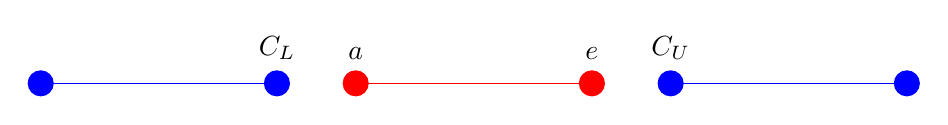
\begin{tikzpicture}[scale=2]
        \coordinate (A) at (0,0);
        \coordinate (B) at (1.5,0);
        \coordinate (C) at (2.0,0);
        \coordinate (D) at (3.5,0);
        \coordinate (E) at (4.0,0);
        \coordinate (F) at (5.5,0);

        \draw[blue] (A) -- (B);
        \draw[red]  (C) -- (D);
        \draw[blue] (E) -- (F);

        \node[circle,fill=blue,radius=0.15]                     at (A) {};
        \node[circle,fill=blue,radius=0.15,label=above : $C_L$] at (B) {};
        \node[circle,fill=red,radius=0.15,label=above  : $a$]   at (C) {};
        \node[circle,fill=red,radius=0.15,label=above  : $e$]   at (D) {};
        \node[circle,fill=blue,radius=0.15,label=above : $C_U$] at (E) {};
        \node[circle,fill=blue,radius=0.15]                     at (F) {};
    \end{tikzpicture}
\end{subfigure}

\par\bigskip

\begin{subfigure}{\textwidth}
    \centering
    \caption{Valid position: $C_L \leq u \leq d \leq e$}
    \label{subfig:all}
    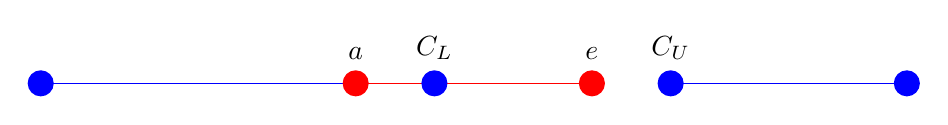
\begin{tikzpicture}[scale=2]
        \coordinate (A) at (0,0);
        \coordinate (B) at (2.5,0);
        \coordinate (C) at (2.0,0);
        \coordinate (D) at (3.5,0);
        \coordinate (E) at (4.0,0);
        \coordinate (F) at (5.5,0);

        \draw[blue] (A) -- (B);
        \draw[red]  (C) -- (D);
        \draw[blue] (E) -- (F);

        \node[circle,fill=blue,radius=0.15]                     at (A) {};
        \node[circle,fill=blue,radius=0.15,label=above : $C_L$] at (B) {};
        \node[circle,fill=red,radius=0.15,label=above  : $a$]   at (C) {};
        \node[circle,fill=red,radius=0.15,label=above  : $e$]   at (D) {};
        \node[circle,fill=blue,radius=0.15,label=above : $C_U$] at (E) {};
        \node[circle,fill=blue,radius=0.15]                     at (F) {};
    \end{tikzpicture}
\end{subfigure}

\par\bigskip

\begin{subfigure}{\textwidth}
    \centering
    \caption{Valid position: $a \leq u \le d \leq C_U$}
    \label{subfig:egu}
    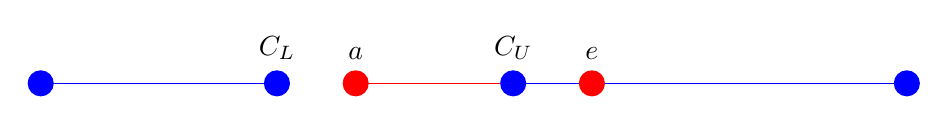
\begin{tikzpicture}[scale=2]
        \coordinate (A) at (0,0);
        \coordinate (B) at (1.5,0);
        \coordinate (C) at (2.0,0);
        \coordinate (D) at (3.5,0);
        \coordinate (E) at (3.0,0);
        \coordinate (F) at (5.5,0);

        \draw[blue] (A) -- (B);
        \draw[red]  (C) -- (D);
        \draw[blue] (E) -- (F);

        \node[circle,fill=blue,radius=0.15]                     at (A) {};
        \node[circle,fill=blue,radius=0.15,label=above : $C_L$] at (B) {};
        \node[circle,fill=red,radius=0.15,label=above  : $a$]   at (C) {};
        \node[circle,fill=red,radius=0.15,label=above  : $e$]   at (D) {};
        \node[circle,fill=blue,radius=0.15,label=above : $C_U$] at (E) {};
        \node[circle,fill=blue,radius=0.15]                     at (F) {};
    \end{tikzpicture}
\end{subfigure}

\par\bigskip

\begin{subfigure}{\textwidth}
    \centering
    \caption{Valid position: $C_L \le u \leq d \leq C_U$}
    \label{subfig:invertsandwhich}
    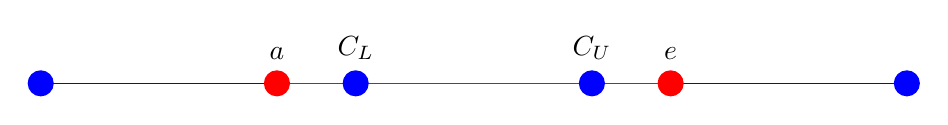
\begin{tikzpicture}[scale=2]
        \coordinate (A) at (0,0);
        \coordinate (B) at (1.5,0);
        \coordinate (C) at (2.0,0);
        \coordinate (D) at (3.5,0);
        \coordinate (E) at (4.0,0);
        \coordinate (F) at (5.5,0);

        \draw[blue] (A) -- (C);
        \draw[blue] (D) -- (F);
        \draw[red]  (B) -- (E);

        \node[circle,fill=blue,radius=0.15]                    at (A) {};
        \node[circle,fill=red,radius=0.15,label=above : $a$]   at (B) {};
        \node[circle,fill=blue,radius=0.15,label=above: $C_L$] at (C) {};
        \node[circle,fill=blue,radius=0.15,label=above: $C_U$] at (D) {};
        \node[circle,fill=red,radius=0.15,label=above : $e$]   at (E) {};
        \node[circle,fill=blue,radius=0.15]                    at (F) {};
    \end{tikzpicture}
\end{subfigure}

\par\bigskip

\begin{subfigure}{\textwidth}
    \centering
    \caption{Invalid position upper bound}
    \label{subfig:invalid-upper}
    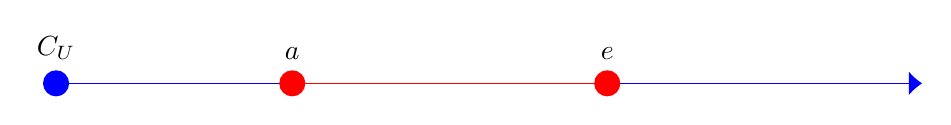
\begin{tikzpicture}[scale=2]
        \coordinate (A) at (0.0,0);
        \coordinate (B) at (5.5,0);
        \coordinate (C) at (1.5,0);
        \coordinate (D) at (3.5,0);

        \draw[-{Latex[width=3mm]},blue]  (A) -- (B);
        \draw[red]  (C) -- (D);

        \node[circle,fill=blue,radius=0.15,label=above : $C_U$] at (A) {};
        \node[circle,fill=red,radius=0.15,label=above  : $a$] at (C) {};
        \node[circle,fill=red,radius=0.15,label=above  : $e$] at (D) {};
    \end{tikzpicture}
\end{subfigure}

\par\bigskip

\begin{subfigure}{\textwidth}
    \centering
    \caption{Invalid position lower bound}
    \label{subfig:invalid-lower}
    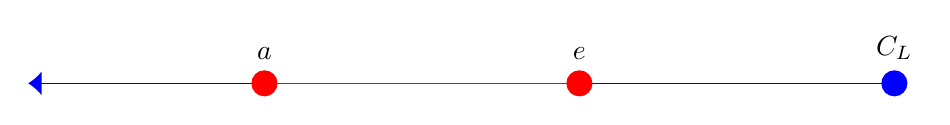
\begin{tikzpicture}[scale=2]
        \coordinate (A) at (0.0,0);
        \coordinate (B) at (5.5,0);
        \coordinate (C) at (1.5,0);
        \coordinate (D) at (3.5,0);

        \draw[-{Latex[width=3mm]},blue]  (B) -- (A);
        \draw[red]  (C) -- (D);

        \node[circle,fill=blue,radius=0.15,label=above : $C_L$] at (B) {};
        \node[circle,fill=red,radius=0.15,label=above  : $a$] at (C) {};
        \node[circle,fill=red,radius=0.15,label=above  : $e$] at (D) {};
    \end{tikzpicture}
\end{subfigure}

\caption{This figure depicts the different states in which a charger with an availability time frame, $[C_L,C_U]$, can be placed on a timeline relative to a visit's total time at the station. The blue lines indicate ranges where the charger is being uilized. The point $C_L$ is the lower bound of the available time and $C_U$ is the upper bound. The red lines, $\bar{ae}$, indicate the time slice in which visit $i$ is at the station. Thus, the BEB may be assigned a charge time anywhere in the range between $C_L$ and $C_U$. For example, \ref{subfig:sandwich} allows the BEB to be charged anywhere in the time range $[a, e]$. \ref{subfig:all} allows a BEB to charge in the time frame $[C_L,e]$. \ref{subfig:egu} allows a BEB to charge in the time frame $[a,C_U]$. \ref{subfig:invertsandwhich} allows charging during the time frame $[C_L,C_U]$. The last two permutations, \ref{subfig:invalid-upper} and \ref{subfig:invalid-lower}, do not allow the BEB to be assigned.}
\label{fig:find-free}
\end{figure}
\begin{algorithm}[H]
\caption{Find free time algorithm checks whether the BEB time at the station, $[a_i, e_i]$ fits within the charger availability $[L,C_U]$. If it does, a random charge time slice is returned, otherwise the null value is returned.}
\label{alg:find-free-time}
    \LinesNumbered
    \TitleOfAlgo{Find Free Time}
    \KwIn{$(C,a,e)$}
    \KwOut{($\bar{C},\bar{u},\bar{d})$}

    \Begin
    { \tcc{Extract the lower and upper bounds.} \(C_L \leftarrow\) \(\{C\}\)\; \(C_U \leftarrow\) \(\{C\}\)\;

      \If(\tcc*[f]{If $C_L \le a \le e \le C_U$ (\autoref{subfig:sandwich})}){$C_L \leq a$ and $C_U \geq e$}
      {
        $\bar{u}\leftarrow$ $\U_{[a,e]}$\;
        $\bar{d}\leftarrow$ $\U_{[\bar{u},e]}$\;
      }
      \ElseIf(\tcc*[f]{Else if $a \le C_L \le e < C_U$ (\autoref{subfig:all})}){$C_L \ge a$ and $C_U \geq e$}
      {
        $\bar{u}\leftarrow$ $\U_{[C_L,e]}$\;
        $\bar{d}\leftarrow$ $\U_{[\bar{u},e]}$\;
      }
      \ElseIf(\tcc*[f]{Else if $C_L \le a \le C_U < e$ (\autoref{subfig:egu})}){$C_L \leq a$ and $C_U \le e$}
      {
        $\bar{u}\leftarrow$ $\U_{[a,C_U]}$\;
        $\bar{d}\leftarrow$ $\U_{[\bar{u},C_U]}$\;
      }
      \ElseIf(\tcc*[f]{Else if $a \leq C_L \leq C_D \leq u$ (\autoref{subfig:invertsandwhich})}){$C_L \ge a$ and $C_U \le e$}
      {
        $\bar{u}\leftarrow$ $\U_{[C_L,C_U]}$\;
        $\bar{d}\leftarrow$ $\U_{[\bar{u},C_U]}$\;
      }
      \Else(\tcc*[f]{Otherwise the bus cannot be scheduled in this time frame (\autoref{subfig:invalid-lower}, \autoref{subfig:invalid-upper})})
      {
        $\bar{u}\leftarrow$ $\varnothing$\;
        $\bar{d}\leftarrow$ $\varnothing$\;
      }

      \If (\tcc*[f]{If an assignment was made}) {$\bar{u},\bar{d} \ne \varnothing$}
      {
        $\bar{C}' \leftarrow C' \cup \{[\bar{u},\bar{d}]\}$\tcc*{Update the compliment of the charger free time slices}
        \Return{($\bar{C},\bar{u},\bar{d}$)}
      }
      \Else(\tcc*[f]{Otherwise the assignment failed})
      {
        \Return{($C,\varnothing, \varnothing$)}
      }
    }
\end{algorithm}

\paragraph{Purge}
\label{sec:purge}
The purge primitive generator simply removes a visit from a charger availability schedule, \(\C\). This generator exists
so that other primitives may place the visit back into the schedule without creating duplicate entries in \(\C\). Line 2
from \ref{alg:purge} updates \(\C\) with the set of visits excluding visit \(i\) from charging queue \(q_i\). Line 3 returns
the updated set of charger availability.

\begin{algorithm}[H]
  \caption{Purge algorithm} \label{alg:purge}
    \LinesNumbered
    \TitleOfAlgo{Purge}
    \KwIn{$\Sol$}
    \KwOut{$\bar{\Sol}$}

    \Begin
    { $\bar{\C} \leftarrow \C \setminus \C_{i.q_i}$\tcc*{Remove assignment of visit $i$ to charger $q_i$} \Return{$(\_,
        \bar{\C})$}\tcc*{Return updated tuple} }
  \end{algorithm}

\paragraph{Slide visit}
\label{slide-visit}
This primitive generator is used for buses that have already been scheduled. Because of the constraint \ref{seq:c8}
there may be some slack to manipulate \([u_i, d_i]\) within the window \([a_i, e_i]\). That is, two new values, \(u_i\) and
\(d_i\) are randomly selected with a uniform distribution that satisfy the constraint \(a_i \leq u_i \leq d_i \leq e_i\). Line 2 from
\ref{alg:slide-visit} purges the visit from the charger availability schedule. Line 4 retrieves the window that was
opened up by purging visit \(i\). Line 4 sets the new charge time frame, \([u_i, d_i]\). Line 5 returns the updated visit
information. If \texttt{findFreeTime} was unsuccessful, then the generator returns a tuple of null values.

\begin{algorithm}[H]
  \caption{Slide Visit Algorithm} \label{alg:slide-visit}
  \LinesNumbered
  \TitleOfAlgo{Slide Visit}
  \KwIn{$\Sol$}
  \KwOut{$\bar{\Sol}$}

    \SetKwFunction{Purge}{Purge}

    \Begin
    {
      $(\_, \bar{\C}) \leftarrow$\Purge{$\Sol$}\tcc*{Purge visit $i$ from charger availibility matrix}
      $C \leftarrow \bar{C}_{i.q_i}$\tcc*{Get the time availability of the purged visit}

        \If(\tcc*[f]{If there is time available in $C$}){($\bar{C}, \bar{u}, \bar{d}$) $\leftarrow$ \findFreeTime{$C$,
            $\I_{i.a}, \I_{i.e}$} $\not\in \varnothing$} { \Return{($\_,
            (\I_{i.q_i},\bar{u},\bar{d}),\bar{C}$)}\tcc*[f]{Return updated visit} }

        \Return{($\varnothing$)}\tcc*{Return nothing}
    }
  \end{algorithm}

\paragraph{New charger}
\label{new-charger}
The new charger generator moves a visit \(\I_i\) to a new charging queue while maintaining the same charge time, \([u_i,
d_i]\). Line 2 from \ref{alg:new-charger} purges the visit from the charger availability set. Line 3 randomly selects a
charger queue index, \(q\). Line 4 checks if there is an available time slice \([a_i, e_i]\) for charger \(q\). Line 5 returns
the updated visit data. If \texttt{findFreetime} was unsuccessful, then the generator returns a tuple of null values.

\begin{algorithm}[H]
  \caption{New Charger Algorithm} \label{alg:new-charger} \LinesNumbered \TitleOfAlgo{New Charger} \KwIn{$\Sol$}
  \KwOut{$\bar{\Sol}$}

    \SetKwFunction{Purge}{Purge}

    \Begin
    {
      $(\_, \bar{\C}) \leftarrow$\Purge{$\Sol$}\tcc*{Purge visit $i$ from charger availibility matrix}
      $q \leftarrow \mathcal{U}_{Q}$\tcc*{Select a random charging queue with a uniform distribution}

      \If(\tcc*[f]{If there is time available in $C_{q}$}){($\bar{C}, \_$) $\leftarrow$ \findFreeTime{$\bar{\C}_{i.q}$, $\I_{i.a}, \I_{i.e}$} $\not\in \varnothing$}
      {
        \tcc{Return visit, note $u$ and $d$ are the original inital/final charge times.}
        \Return{($\_, (q,\I_{i.u}, \I_{i.d}),\bar{\C}$)}
      }

      \Return{($\varnothing$)}\tcc*{Return nothing}
    }
  \end{algorithm}

\paragraph{Wait}
\label{sec:wait}
The wait generator simply removes a bus from a charger queue and places it in its idle queue, \(q_i \in \{1,...,B\}\).
Line 2 from \ref{alg:wait} purges the visit from the charger availability set. Line 4 updates the complement charger
availability schedule of the wait queue for bus \(b\). Line 5 returns the updated visit. Line 7 returns the null set upon
failure of assignment.

\begin{algorithm}[H]
\caption{Wait algorithm} \label{alg:wait}
    \LinesNumbered
    \TitleOfAlgo{Wait}
    \KwIn{$\Sol$}
    \KwOut{$\bar{\Sol}$}

    \SetKwFunction{Purge}{Purge}

    \Begin
    { $(\_, \bar{\C}) \leftarrow$\Purge{$\Sol$}\tcc*{Purge visit $i$ from charger availibility matrix}
      $\bar{\C}'_{\I_{i.\Gamma_i}} \leftarrow \C' \cup \{[\I_{i.a}, \I_{i.e}]\}$\tcc*{Update the charger availability
        matrix for wait queue $\bar{\C}_{i.q_i}$} \Return{$(\_, (\I_{i.b}, \I_{i.a}, \I_{i.e}),
        \bar{\C})$}\tcc*[f]{Return visit} }
  \end{algorithm}

\paragraph{New Window}
\label{sec:new-window}
New window is a combination of \ref{alg:new-visit} (new visit) and \ref{alg:purge} (purge). By this it is meant that
visit \(i\) is purged and added back in as if it were a new visit. This implies that the BEB may be assigned to a
different queue and a new charge time slice. Line 2 purges the BEB visit from the schedule producing \(\bar{\Sol}\). Line
3 places the BEB back into the schedule using the new visit generator, producing \(\bar{\bar{\Sol}}\). Line 4 assigns and
returns the updated visit. Line 6 returns the null visit upon failure of \ref{alg:new-visit}.

\begin{algorithm}[H]
  \caption{New window algorithm} \label{alg:new-window}
  \LinesNumbered
  \TitleOfAlgo{New Window}
  \KwIn{$\Sol$}
  \KwOut{$\bar{\Sol}$}

  \SetKwFunction{NewVisit}{NewVisit}
  \SetKwFunction{Purge}{Purge}

  \Begin
  {
    $\bar{\Sol} \leftarrow$\Purge{$\Sol$}\tcc*{Purge visit $i$ from charger availibility matrix}
    \If(\tcc*[f]{Add visit $i$ back in randomly})
       {
         $\bar{\bar{\Sol}} \leftarrow$ \NewVisit{$\bar{\Sol}$} $\not\in \varnothing$
       }
       {
         \Return{$\bar{\bar{\Sol}}$} \tcc*[f]{Return visit}
       }

       \Return{($\varnothing$)}\tcc*{Return nothing}
  }
\end{algorithm}

\subsubsection{Generator Wrappers}
\label{sec:generator-wrappers}
This section covers the algorithms utilized to select and execute different generation processes. The generator wrappers
are the methods immediately called by the SA algorithm. Each wrapper utilizes the primitive generators previously
described and returns either a new charge schedule or a modified charge schedule.

\paragraph{Charge Schedule Generation}
\label{sec:charge-schedule-generation}
The objective of this generator is to assign each BEB to its idle queue provided a schedule of routes. Specifically,
this generator exists to initialize the system with a solution that is spatiotemporally feasible, but does not satisfy
the battery dynamic constraints. This problem is addressed by the penalty method by allowing the infeasible battery SOCs
to occur, but penalizing the system for doing so. Line 2 of \ref{alg:charge-schedule-generation} loops through each
visit and Line 4 executes \ref{alg:wait}.

\begin{algorithm}[H]
\caption{Charge schedule generation algorithm} \label{alg:charge-schedule-generation}
    \LinesNumbered
    \TitleOfAlgo{Candidate Solution Generator}
    \KwIn{$\I$, $\C$}
    \KwOut{$\bar{\I}$, $\bar{\C}$}

    \SetKwFunction{Wait}{Wait}

    \Begin
    {
        \tcc{Select an unscheduled BEB visit from a randomly indexed set of visits}
        \ForEach {$\I_i \in \I$}
        {
            (\_, $\bar{\I}$, $\bar{\C}$) $\leftarrow$ \Wait{($\I_i$, $\I$, $\C$)}\tcc*{Assign the bus to a charger}
        }
            \Return{($\bar{\I}$, $\bar{\C}$)}
    }
  \end{algorithm}

\paragraph{Perturb Schedule}
\label{sec:tweak-schedule}
Once the active solution has been created by \ref{alg:charge-schedule-generation}, the SA process begins modifying it to
create candidate solutions. After each step of the cooling function, the active solution will be altered \(n_k\) times by
a random primitive generator. During these \(n_k\) iterations the active solution is modified to create a neighboring
candidate solution. This candidate solution will then be compared against the active solution in the manner discussed in
\ref{sec:acceptance}. This algorithm describes the method by which the SA algorithm decides how to perturb the schedule. The
method that will be employed generate a neighboring solution is as follows: pick a visit, pick a primitive generator,
and execute said primitive generator once. Thus, \ref{alg:perturb-schedule} is as follows: Line 2 selects a visit at
random with a uniform distribution. Line 3 extracts the visit index. Letting \(n_G\) denote the number of primitive
generating functions, Line 4 selects a primitive generator. Line 5 executes the primitive, and Line 6 returns the
result.

\begin{algorithm}[H]
\caption{Perturb schedule algorithm} \label{alg:perturb-schedule}

    \LinesNumbered
    \TitleOfAlgo{Perturb Schedule}
    \KwIn{$\I$, $\C$}
    \KwOut{$\bar{\I}$, $\bar{\C}$}

    \SetKwFunction{PGF}{PGF}

    \Begin
    {
        $\I_i\leftarrow\; \U_{\I}$\tcc*{Randomly select a visit}
        $i \leftarrow\; \I_i$\tcc*{Extract visit index}
        $PGF \leftarrow\; \U_{[1,n_G]}$\tcc*{Select one of the generator functions}
        $\bar{\Sol} \leftarrow$ \PGF{($i$, $\I$, $\C$)}\tcc*{Excecute the generator function}
        \Return{($\_, \bar{\I}$, $\bar{\C}$)}
    }
\end{algorithm}
\section{Optimization Algorithm}
\label{sec:optimization-algorithm}
This section combines the generation algorithms and the optimization problem into a single algorithm. It begins with an
introduction and discussion of a general SA algorithm which will be used to springboard into the construction of the SA
PAP algorithm.

\subsection{Simulated Annealing Pseudo Code}
\label{sec:simulated-annealing-pseudo-code}
Let \(\omega\) and \(\bar{\omega}\) denote the active solution and
the candidate solution, respectively. Let \(\Tau\) be the temperature function and \(\Tau_0\) the initial temperature.
Furthermore, let \(t\) be defined as the vector of temperatures defined by \(t = \Tau(\Tau_0)\), and let \(t_m\) be defined as
being an element of \(t\), \(t_m \in t\). Let \(n_K\) be the repetition counter, it defines the number of iterations to execute
exploit a solution at a constant temperature \(t_m\).

Recall the objective of the SA algorithm is to iteratively create a neighboring candidate solution from the active
solution. The fitness of the two solutions are compared and if the candidate solution is of a higher quality, it is
always taken as the active solution. If it is not, then it may be selected as the new candidate solution with some
probability that is a function of the difference in the objective function values and the current temperature. This
process is iteratively done until the temperature function reaches its minimum value. With the high level summary in
mind, the SA pseudocode is to be presented \cite{henderson-1989-theor-pract}.

The algorithm behaves as follows: Lines 1 and 2 of \ref{alg:sa-pseudo} initialize the SA algorithm an active solution,
\(\omega\), and temperature schedule, \(t\), respectively. The outer loop on Line 3 iterates through all the temperature values
in \(t\). After each iteration of the outer loop, the temperature is decreased as specified by the selected temperature
function. Line 4 resets the iteration counter to 0. Line 5 specifies the inner loop that iterates \(n_K\) times at a
constant temperature, \(t_k\). Line 6, perturbs the active solution \(\omega\) to a neighboring candidate solution \(\bar{\omega} =
N(\omega)\). Line 7 then calculates the difference in the fitness of \(\omega\) and \(\bar{\omega}\). Lines 8-13 updates \(\omega\) with \(\bar{\omega}\)
if the candidate solution is more fit, or updates \(\omega\) with \(\bar{\omega}\) with probability \(e^{\frac{-\Delta_{\omega , \bar{\omega}}}{t_m}}\)
if the candidate solution is less fit than the active solution. Line 14 updates the repetition counter.

\begin{algorithm}[H]
\caption{Pseudo-code for SA} \label{alg:sa-pseudo}
    \LinesNumbered
    \TitleOfAlgo{SA Pseudo-Code}

    \SetKwFunction{Obj}{J}
    \SetKwFunction{New}{N}
    \SetKwFunction{Pert}{P}
    \SetKwFunction{Temp}{$\Tau$}

    \Begin
    {
        $\omega \leftarrow$ \New{($\I$, $\C$)}\tcc*{Generate an initial solution}
        \tcc{Generate vector of temperatures given temperature function $\Tau$ and initial temperature $\Tau_0$}
        $t \leftarrow$ \Temp{$\Tau_0$}

        \ForEach{$t_m \in t$}
        {
          $k \leftarrow 0$ \tcc*{Initialize repetition counter}

          \While{$k \le n_K$}
          {
            $\bar{\omega} \leftarrow $ \Pert{($\I$, $\C$)}\tcc*{Perturb the solution}
            $\Omega_{\bar{\omega},\omega} \rightarrow$ \Obj{$\bar{\omega}$} - \Obj{$\omega$}\tcc*{Calculate the difference of fitness scores}

            \tcc{Compare and update current solution}
            \If{$\Omega_{\bar{\omega},\omega} \le 0$}{$\omega \leftarrow \bar{\omega}$}
            \If{$\Omega_{\bar{\omega},\omega} > 0$}{$\omega \leftarrow \bar{\omega}$ with probability $e^{\frac{-\Omega_{\bar{\omega},\omega}}{t_m}}$}

            $k \leftarrow k+1$\tcc*{Increment the reptition counter}
          }
        }
    }
\end{algorithm}

\subsection{SA PAP Pseudo Code}
\label{sec:sa-pap-pseudo-code}
Now that the general SA algorithm has been outlined, the objective is now to outline SA-PAP (\ref{alg:sa-pap}). While
the SA PAP generally is written almost identically to that of the general SA algorithm, the general SA assumes that the
generated candidate solutions are in the solution space of the problem, \(\omega \in S\) where \(S\) is the solution space.
Initialization and the perturbation of a schedule must be verified to ensure that the generated schedule is in the
solution space. Therefore, the objective function and constraints introduced in \ref{sec:constraints} and
\ref{sec:objective-function}, respectively, must be employed to verify that the output of
\ref{alg:charge-schedule-generation} is in the feasible space, \(S\).

As previously stated, the generating functions directly influence the values of the assigned charge queue, charge
initialization time, and charge completion time: \(q_i\), \(u_i\), and \(d_i\), respectively. Having generated those values,
the rest of the decision variables may be derived. Let's begin by reviewing over the packing constraints.
\ref{seq:c0}-\ref{seq:c1} are employed to enable and disable \(\sigma_{ij}\) and \(\psi_{ij}\) and \ref{seq:c2}-\ref{seq:c4} ensure
the validity of the values. \ref{seq:c5} can be directly calculated and \ref{seq:c8} is fully defined.

Now let's change the focus over to the dynamic constraints. Similar to what was seen with the packing constraints, the
battery dynamic constraints are also fully defined and can be calculated. \ref{seq:c6} is sequentially calculated after
a given schedule has been fully defined. \ref{seq:c7} is evaluated to ensure the BEB is not overcharged. The penalty
method implemented in \ref{sec:objective-function} is set in place to allow the SOC to go below the specified threshold,
\(\nu_{\Xi_i} \kappa_{\Xi_i}\), but punish the solution for doing so. Thus, over time, the candidate solutions will be encouraged
toward a solution that does not activate the penalty method (i.e. is solution is truly feasible).

The SA-PAP algorithm will now be outlined. Line 2 initializes the SA algorithm by creating a vector of temperature
values based on a temperature schedule \(\Tau\), and initial temperature \(\Tau_0\). Line 3 generates the initial candidate
solution \(\omega\), note that \(CSG(\cdot)\) (candidate solution generator) is used to denote the specific candidate solution
generator being utilized. For SA PAP it is \ref{alg:charge-schedule-generation}. Line 4 loops through each of the step
in the temperature schedule \(t_m \in t\). Line 5 resets the iteration count to 0. Line 6 specifies the inner loop that
iterates \(n_K\) times at a constant temperature, \(t_k\). Line 7, perturbs the active solution \(\omega\) to a neighboring
candidate solution \(\bar{\omega} = PS(\omega)\), where \(PS(\cdot)\) (perturb schedule) is \ref{alg:perturb-schedule}. Line 8 calculates
the difference in the fitness of \(\omega\) and \(\bar{\omega}\). Lines 8-14 are similar to \ref{alg:sa-pseudo} where it updates \(\omega\)
with \(\bar{\omega}\) if the candidate solution is more fit, or updates \(\omega\) with \(\bar{\omega}\) with probability
\(e^{\frac{-\Delta_{\bar{\omega},\omega}}{t_m}}\) if the candidate solution is less fit than the active solution. What makes these lines
unique is that the active solution is only updated if the candidate is within the solution space. That it, it satisfies
the constraints defined in \ref{eq:constraints}.

\begin{algorithm}[H]
  \caption{Simulated annealing approach to the position allocation problem} \label{alg:sa-pap}
  \LinesNumbered
  \TitleOfAlgo{SA PAP}
  \KwIn{($\I$ , $\C$)}
  \KwOut{($\bar{\I}$, $\bar{\C}$)}

  \SetKwFunction{Temp}{$\Tau$}
  \SetKwFunction{CSG}{CSG}
  \SetKwFunction{PS}{PS}
  \SetKwFunction{Obj}{J}

  \Begin
    {
      \tcc{Generate vector of temperatures given temperature function $\Tau$ and initial temperature $\Tau_0$}
      $t \leftarrow$ \Temp{$\Tau_0$}

      $\omega \leftarrow$\CSG{($\I$, $\C$)}\tcc{Generate an initial solution}

      \tcc{For each item in the temperature vector}
      \ForEach{$t_k \in t$}
       {
         $k \leftarrow 0$\tcc*{Initialize repetition counter}

        \tcc{For each step in the repitition schedule}
        \While{$k \le n_K$}
        {
          $\bar{\omega} \leftarrow$ \PS{($\I$, $\C$)} \tcc*{Generate a new solution}
          $\Omega_{\bar{\omega},\omega} = $ \Obj{$\bar{\omega}$}  - \Obj{$\omega$} \tcc*{Calculate the difference of fitness scores}

          \If{$\bar{\I} \in S$ and $\Omega_{\bar{\omega},\omega} \le 0$}{$\omega \leftarrow \bar{\omega}$}
          \If{$\bar{\I} \in S$ and $\Omega_{\bar{\omega},\omega} > 0$}{$\omega \leftarrow \bar{\omega}$ with probability $e^{\frac{\Omega_{\omega, \bar{\omega}}}{t_k}}$}

          $k \leftarrow k+1$\tcc*{Increment the reptition counter}
        } % For k
      }   % For t_k \in t

      \Return{($\bar{\I}$ , $\bar{\C}$)}
    } % Begin
\end{algorithm}

\section{Example}
\label{sec:example}
An example is now provided to demonstrate the utility of the developed SA charge scheduling technique. A description of
the scenario presented followed by a brief introduction of the original MILP-PAP implementation as well as an
alternative heuristic based planning strategy called Quin-Modified which is used as a comparison to the SA PAP. Results
are then presented for each of planning strategies are presented, analyzed, and discussed.

\subsection{BEB Scenario}
\label{beb-scenario}
To display the capabilities of the model, an example scenario is presented. The scenario was run over a time horizon of
\(T=24\) hours, utilizes \(n_B = \A\) buses with \(n_V = \N\) visits to the station divided between the \(n_B\) buses. As stated
before, the route times are sampled from a set of routes from the UTA. Each bus has \batsize KWh battery that is
required to stay above \mincharge charge (\fpeval{\batsize * \minchargeD} KWh) to maintain battery health. Each bus is
assumed to begin the working day with \fpeval{\acharge*100}\% charge (\fpeval{\acharge * \batsize} KWh). Additionally,
each bus is required to end the day with a minimum charge of \fpeval{\bcharge * 100}\% (\fpeval{\bcharge * \batsize}
KWh). This assumes that overnight charging can account for at least 20\% of the charge. Each bus is assumed to discharge
at a rate of 30 KW. Note that there are many factors that play a role in the rate of discharge; however, for the sake of
simplicity an average rate is used. \(n_C =\) \fpeval{\fast + \slow} chargers are utilized where \slow of the chargers are
slow charging (\slows KW) and \fast are fast charging (\fasts KW). A technique to minimize chargers will be employed.

To encourage the SA PAP problem to utilize the fewest number of chargers, the value of \(m_q\) in the objective function
is \(\forall q \in \{1,2,..., n_B \}; m_q = 0\) and \(\forall q \in \{n_b + 1, n_b + 2,..., n_Q \}; m_q = 1000q\). The charge duration
scalar, \(\epsilon_q\), is defined as \(\epsilon_q = r_q\) to create a consumption cost term, \(g_{iq}\epsilon_q\). This is utilized to also
encourage the model to minimize active charger times, particularly for the fast chargers.

Another heuristic-based optimization strategy, referred to as Quin-Modified, is also employed as a means of comparison
with the results of the SA PAP. The Quin-Modified strategies is a based on the threshold strategy of
\cite{qin-2016-numer-analy}. The strategy has been modified slightly to accommodate the case of multiple charger types
and without exhaustive search for the best charger type. The heuristic is based on a set of rules that revolve around
the initial charge of the bus at visit \(i\). There are three different thresholds, low (85\%), medium (90\%), and high
(95\%). Buses below the low threshold are prioritized to fast chargers then are allowed to utilize slow chargers if no
fast chargers are available. Buses between the low and medium threshold prioritize slow chargers first and utilize fast
chargers only if no slow chargers are available. Buses above the medium threshold and below high will only be assigned
to slow chargers. Buses above the high threshold will not be charged. Once a bus has been assigned to a charger, it
remains on the charger for the duration of the time it is at the station, or it reaches 95\% charge, whichever comes
first.

UTA bus routing data that occurs over a 24-hour time period. The optimization was performed using a machine running an
AMD Ryzen 9 5900X 12 - Processor (24 core) at 4.95GHz. The solver was allowed to run for \timeran hours.

\begin{subfigures}
%%~~~~~~~~~~~~~~~~~~~~~~~~~~~~~~~~~~~~~~~~~~~~~~~~~~~~~~~~~~~~~~~~~~~~~~~~~~~~
% Quinn
    \begin{figure}[htpb]
    \centering \includegraphics{sections/img/schedule-quinn}
        \caption{Charging schedule generated by Quin Modified algorithm.}
        \label{subfig:schedule-quin}
    \end{figure}

    \hfill

   %%~~~~~~~~~~~~~~~~~~~~~~~~~~~~~~~~~~~~~~~~~~~~~~~~~~~~~~~~~~~~~~~~~~~~~~~~~~~~
   % MILP
   \begin{figure}[htpb]
   \centering \includegraphics{sections/img/schedule-milp}
       \caption{Charging schedule generated by MILP PAP algorithm.}
       \label{subfig:schedule-milp}
   \end{figure}

   %%~~~~~~~~~~~~~~~~~~~~~~~~~~~~~~~~~~~~~~~~~~~~~~~~~~~~~~~~~~~~~~~~~~~~~~~~~~~~
   % SA
   \begin{figure}[htpb]
   \centering \includegraphics{sections/img/schedule-sa}
       \caption{Charging schedule generated by SA PAP algorithm.}
       \label{subfig:schedule-sa}
   \end{figure}
\end{subfigures}

\begin{subfigures}
    %%~~~~~~~~~~~~~~~~~~~~~~~~~~~~~~~~~~~~~~~~~~~~~~~~~~~~~~~~~~~~~~~~~~~~~~~~~~~~
    % Fast
    \begin{figure}[htpb]
    \centering
        \includegraphics{sections/img/charger-count-fast}
        \caption{Number of fast chargers for Quin and MILP PAP.}
        \label{subfig:fast-charger-usage}
    \end{figure}

    \hfill

    %%~~~~~~~~~~~~~~~~~~~~~~~~~~~~~~~~~~~~~~~~~~~~~~~~~~~~~~~~~~~~~~~~~~~~~~~~~~~~
    % Slow
    \begin{figure}[!ht]
    \centering
        \includegraphics{sections/img/charger-count-slow}
        \caption{Number of slow chargers for Quin and MILP PAP.}
        \label{subfig:slow-charger-usage}
    \end{figure}
\end{subfigures}

\begin{subfigures}
    %%~~~~~~~~~~~~~~~~~~~~~~~~~~~~~~~~~~~~~~~~~~~~~~~~~~~~~~~~~~~~~~~~~~~~~~~~~~~~
    % Quinn
    \begin{figure}[htpb]
    \centering
        \includegraphics{sections/img/charge-quinn}
        \caption{Bus charges for the Quin Modified charging schedule. The charging scheme of the Quin charger is more predictable during the working day.}
        \label{subfig:quin-charge}
    \end{figure}

    \hfill

    %%~~~~~~~~~~~~~~~~~~~~~~~~~~~~~~~~~~~~~~~~~~~~~~~~~~~~~~~~~~~~~~~~~~~~~~~~~~~~
    % MILP
    \begin{figure}[htpb]
    \centering
        \includegraphics{sections/img/charge-milp}
        \caption{The bus charges for the MILP PAP charging schedule. The MILP model allows for guarantees of minimum/maximum changes during the working day as well as charges at the end of the day.}
        \label{subfig:milp-charge}
    \end{figure}

    %%~~~~~~~~~~~~~~~~~~~~~~~~~~~~~~~~~~~~~~~~~~~~~~~~~~~~~~~~~~~~~~~~~~~~~~~~~~~~
    % SA
    \begin{figure}[htpb]
    \centering
        \includegraphics{sections/img/charge-sa}
        \caption{The bus charges for the SA PAP charging schedule. The SA model allows for guarantees of minimum/maximum changes during the working day as well as charges at the end of the day.}
        \label{subfig:sa-charge}
    \end{figure}
\end{subfigures}

\begin{figure}[htpb]
\centering
    \includegraphics{sections/img/power}
    \caption{Amount of power consumed by Quin-Modified and MILP schedule over the time horizon.}
    \label{fig:power-usage}
\end{figure}

\begin{figure}[htpb]
\centering \includegraphics{sections/img/energy}
    \caption{Total accumulated energy consumed by the Quin-Modified and MILP schedule throughout the time horizon.}
    \label{fig:energy-usage}
\end{figure}


\bibliographystyle{plain}
\bibliography{c:/msys64/home/1556048963C/Documents/citation-database/lit-ref,c:/msys64/home/1556048963C/Documents/citation-database/lib-ref}
\end{document}